% Options for packages loaded elsewhere
\PassOptionsToPackage{unicode}{hyperref}
\PassOptionsToPackage{hyphens}{url}
\documentclass[
  11pt]{article}
\usepackage{xcolor}
\usepackage[a4paper,margin=1in]{geometry}
\usepackage{amsmath,amssymb}
\setcounter{secnumdepth}{3}
\usepackage{iftex}
\ifPDFTeX
  \usepackage[T1]{fontenc}
  \usepackage[utf8]{inputenc}
  \usepackage{textcomp} % provide euro and other symbols
\else % if luatex or xetex
  \usepackage{unicode-math} % this also loads fontspec
  \defaultfontfeatures{Scale=MatchLowercase}
  \defaultfontfeatures[\rmfamily]{Ligatures=TeX,Scale=1}
\fi
\usepackage{lmodern}
\ifPDFTeX\else
  % xetex/luatex font selection
  \setmainfont[]{TeX Gyre Termes}
  \setmathfont[]{TeX Gyre Termes Math}
\fi
% Use upquote if available, for straight quotes in verbatim environments
\IfFileExists{upquote.sty}{\usepackage{upquote}}{}
\IfFileExists{microtype.sty}{% use microtype if available
  \usepackage[]{microtype}
  \UseMicrotypeSet[protrusion]{basicmath} % disable protrusion for tt fonts
}{}
\makeatletter
\@ifundefined{KOMAClassName}{% if non-KOMA class
  \IfFileExists{parskip.sty}{%
    \usepackage{parskip}
  }{% else
    \setlength{\parindent}{0pt}
    \setlength{\parskip}{6pt plus 2pt minus 1pt}}
}{% if KOMA class
  \KOMAoptions{parskip=half}}
\makeatother
\usepackage{color}
\usepackage{fancyvrb}
\newcommand{\VerbBar}{|}
\newcommand{\VERB}{\Verb[commandchars=\\\{\}]}
\DefineVerbatimEnvironment{Highlighting}{Verbatim}{commandchars=\\\{\}}
% Add ',fontsize=\small' for more characters per line
\newenvironment{Shaded}{}{}
\newcommand{\AlertTok}[1]{\textcolor[rgb]{1.00,0.00,0.00}{\textbf{#1}}}
\newcommand{\AnnotationTok}[1]{\textcolor[rgb]{0.38,0.63,0.69}{\textbf{\textit{#1}}}}
\newcommand{\AttributeTok}[1]{\textcolor[rgb]{0.49,0.56,0.16}{#1}}
\newcommand{\BaseNTok}[1]{\textcolor[rgb]{0.25,0.63,0.44}{#1}}
\newcommand{\BuiltInTok}[1]{\textcolor[rgb]{0.00,0.50,0.00}{#1}}
\newcommand{\CharTok}[1]{\textcolor[rgb]{0.25,0.44,0.63}{#1}}
\newcommand{\CommentTok}[1]{\textcolor[rgb]{0.38,0.63,0.69}{\textit{#1}}}
\newcommand{\CommentVarTok}[1]{\textcolor[rgb]{0.38,0.63,0.69}{\textbf{\textit{#1}}}}
\newcommand{\ConstantTok}[1]{\textcolor[rgb]{0.53,0.00,0.00}{#1}}
\newcommand{\ControlFlowTok}[1]{\textcolor[rgb]{0.00,0.44,0.13}{\textbf{#1}}}
\newcommand{\DataTypeTok}[1]{\textcolor[rgb]{0.56,0.13,0.00}{#1}}
\newcommand{\DecValTok}[1]{\textcolor[rgb]{0.25,0.63,0.44}{#1}}
\newcommand{\DocumentationTok}[1]{\textcolor[rgb]{0.73,0.13,0.13}{\textit{#1}}}
\newcommand{\ErrorTok}[1]{\textcolor[rgb]{1.00,0.00,0.00}{\textbf{#1}}}
\newcommand{\ExtensionTok}[1]{#1}
\newcommand{\FloatTok}[1]{\textcolor[rgb]{0.25,0.63,0.44}{#1}}
\newcommand{\FunctionTok}[1]{\textcolor[rgb]{0.02,0.16,0.49}{#1}}
\newcommand{\ImportTok}[1]{\textcolor[rgb]{0.00,0.50,0.00}{\textbf{#1}}}
\newcommand{\InformationTok}[1]{\textcolor[rgb]{0.38,0.63,0.69}{\textbf{\textit{#1}}}}
\newcommand{\KeywordTok}[1]{\textcolor[rgb]{0.00,0.44,0.13}{\textbf{#1}}}
\newcommand{\NormalTok}[1]{#1}
\newcommand{\OperatorTok}[1]{\textcolor[rgb]{0.40,0.40,0.40}{#1}}
\newcommand{\OtherTok}[1]{\textcolor[rgb]{0.00,0.44,0.13}{#1}}
\newcommand{\PreprocessorTok}[1]{\textcolor[rgb]{0.74,0.48,0.00}{#1}}
\newcommand{\RegionMarkerTok}[1]{#1}
\newcommand{\SpecialCharTok}[1]{\textcolor[rgb]{0.25,0.44,0.63}{#1}}
\newcommand{\SpecialStringTok}[1]{\textcolor[rgb]{0.73,0.40,0.53}{#1}}
\newcommand{\StringTok}[1]{\textcolor[rgb]{0.25,0.44,0.63}{#1}}
\newcommand{\VariableTok}[1]{\textcolor[rgb]{0.10,0.09,0.49}{#1}}
\newcommand{\VerbatimStringTok}[1]{\textcolor[rgb]{0.25,0.44,0.63}{#1}}
\newcommand{\WarningTok}[1]{\textcolor[rgb]{0.38,0.63,0.69}{\textbf{\textit{#1}}}}
\usepackage{graphicx}
\makeatletter
\newsavebox\pandoc@box
\newcommand*\pandocbounded[1]{% scales image to fit in text height/width
  \sbox\pandoc@box{#1}%
  \Gscale@div\@tempa{\textheight}{\dimexpr\ht\pandoc@box+\dp\pandoc@box\relax}%
  \Gscale@div\@tempb{\linewidth}{\wd\pandoc@box}%
  \ifdim\@tempb\p@<\@tempa\p@\let\@tempa\@tempb\fi% select the smaller of both
  \ifdim\@tempa\p@<\p@\scalebox{\@tempa}{\usebox\pandoc@box}%
  \else\usebox{\pandoc@box}%
  \fi%
}
% Set default figure placement to htbp
\def\fps@figure{htbp}
\makeatother
% definitions for citeproc citations
\NewDocumentCommand\citeproctext{}{}
\NewDocumentCommand\citeproc{mm}{%
  \begingroup\def\citeproctext{#2}\cite{#1}\endgroup}
\makeatletter
 % allow citations to break across lines
 \let\@cite@ofmt\@firstofone
 % avoid brackets around text for \cite:
 \def\@biblabel#1{}
 \def\@cite#1#2{{#1\if@tempswa , #2\fi}}
\makeatother
\newlength{\cslhangindent}
\setlength{\cslhangindent}{1.5em}
\newlength{\csllabelwidth}
\setlength{\csllabelwidth}{3em}
\newenvironment{CSLReferences}[2] % #1 hanging-indent, #2 entry-spacing
 {\begin{list}{}{%
  \setlength{\itemindent}{0pt}
  \setlength{\leftmargin}{0pt}
  \setlength{\parsep}{0pt}
  % turn on hanging indent if param 1 is 1
  \ifodd #1
   \setlength{\leftmargin}{\cslhangindent}
   \setlength{\itemindent}{-1\cslhangindent}
  \fi
  % set entry spacing
  \setlength{\itemsep}{#2\baselineskip}}}
 {\end{list}}
\usepackage{calc}
\newcommand{\CSLBlock}[1]{\hfill\break\parbox[t]{\linewidth}{\strut\ignorespaces#1\strut}}
\newcommand{\CSLLeftMargin}[1]{\parbox[t]{\csllabelwidth}{\strut#1\strut}}
\newcommand{\CSLRightInline}[1]{\parbox[t]{\linewidth - \csllabelwidth}{\strut#1\strut}}
\newcommand{\CSLIndent}[1]{\hspace{\cslhangindent}#1}
\setlength{\emergencystretch}{3em} % prevent overfull lines
\providecommand{\tightlist}{%
  \setlength{\itemsep}{0pt}\setlength{\parskip}{0pt}}
\usepackage[most]{tcolorbox}
\usepackage{enumitem}
\usepackage{tabularx}
\usepackage{booktabs}
\usepackage{caption}
\usepackage{float}
\usepackage{etoolbox}
\usepackage{xcolor}
\setlength{\parskip}{0.45em}
\setlength{\parindent}{1.2em}
\setlist[itemize]{leftmargin=1.6em}
\captionsetup[table]{font=small, labelfont=bf, labelsep=period, skip=4pt}
\definecolor{aegray}{HTML}{6E6E6E}
\definecolor{aelight}{HTML}{F3F4F6}
\definecolor{aeline}{HTML}{D7D9DC}
\definecolor{aecite}{HTML}{7A3EF0}
\usepackage{bookmark}
\IfFileExists{xurl.sty}{\usepackage{xurl}}{} % add URL line breaks if available
\urlstyle{same}
\hypersetup{
  hidelinks,
  pdfcreator={LaTeX via pandoc}}

\author{}
\date{}

\begin{document}

\begin{center}
\begin{minipage}{0.94\textwidth}
\centering
\Large\bfseries SCADA-Anchored Regime-Aware Routing for Auditable Wind-Turbine Control-Boundary Forecasting\par
\vspace{0.6em}
\normalsize Junyu Li\textsuperscript{a}\qquad Juntao Du\textsuperscript{a,*}\par
\vspace{0.35em}
\small \textsuperscript{a} School of Statistics and Applied Mathematics, Anhui University of Finance and Economics, Bengbu, 233030, China\par
\end{minipage}
\end{center}

\vspace{0.05em}

\noindent{\scriptsize *Corresponding author.\par}
\noindent{\scriptsize Email addresses: \texttt{ljylikezmn999@gmail.com} (Junyu Li), \texttt{dujuntao@aufe.edu.cn} (Juntao Du)\par}

\vspace{0.35em}

\noindent{\small\bfseries Abstract\par} \vspace{0.18em} \small We
present a framework that makes the wind-turbine MPPT-to-pitch control
boundary auditable through SCADA-anchored, regime-aware routing. Current
spatio-temporal forecasters minimize fleet-average error but do not
assign responsibility to the operating state that generated a local
response. We constrain a node-level mixture-of-experts gate with SCADA
operating anchors so that each sample's routing assignment can be
compared against a declared MPPT-to-pitch partition and then used when
threshold labels are delayed, missing, or noisy. On the KDD Cup 2022
benchmark, the boundary-forced router recovers the declared partition
(NMI about 0.87, ARI about 0.92) at a measured accuracy cost: overall
RMSE 236.13 versus 225.74 for Graph WaveNet. More importantly for
operators, under a six-step label delay the gate retains 0.960 early
pitch-window recall while the delayed threshold rule falls to 0.196;
with only 50\% label availability, the gate remains at 0.960 versus
0.508 for the available-label rule. The same gate exposes where reserve
risk concentrates in the transition window, though validation-frozen
quantile baselines show that physical-bin policies remain competitive.
Kelmarsh/Penmanshiel external tests do not pass the held-out routing
criterion; instead they define a deployment protocol---sensor coverage,
pitch observability, local boundary re-estimation, and held-out routing
checks---that must be satisfied before cross-farm use. The contribution
is an auditable control-boundary routing framework with quantified
degraded-label value, measured RMSE price, and explicit cross-site
transfer conditions, not a claim of forecasting superiority or universal
reserve-policy optimality.

\vspace{0.25em}

\noindent{\small\textbf{Keywords:} Wind-turbine control boundary; SCADA-anchored routing; regime-aware forecasting; auditable routing; MPPT-to-pitch transition; mixture-of-experts.\par}

\normalsize

\vspace{0.55em}

\section*{Highlights}\label{highlights}
\addcontentsline{toc}{section}{Highlights}

\begin{itemize}
\tightlist
\item
  SCADA anchors make the MPPT-to-pitch control boundary auditable
  through routing.
\item
  Regime gates recover the declared partition (NMI 0.87) at a measured
  RMSE cost.
\item
  The gate keeps early pitch-window recall under delayed or missing
  threshold labels.
\item
  Validation-frozen quantile baselines bound any reserve-policy claim
  honestly.
\item
  External-site tests define deployment gates, not automatic cross-farm
  transfer.
\end{itemize}

\section*{Nomenclature}\label{nomenclature}
\addcontentsline{toc}{section}{Nomenclature}

\begin{table}[H]
\centering
\footnotesize
\setlength{\tabcolsep}{5pt}
\renewcommand{\arraystretch}{1.08}
\caption*{\textbf{Nomenclature.} Core symbols, variables, and abbreviations.}
\begin{tabularx}{0.98\linewidth}{>{\raggedright\arraybackslash}p{0.18\linewidth} >{\raggedright\arraybackslash}X}
\toprule
Symbol or term & Meaning \\
\midrule
$G=(V,E)$ & Wind-farm or grid graph with nodes $V$ and edges $E$ \\
$N$ & Number of turbines or grid nodes \\
$H$, $P$ & Input history length and forecast horizon length \\
$\mathbf{x}_{i,t}$, $y_{i,t}$ & Node feature vector and scalar active-power target \\
$\hat{y}_{i,t}$ & Forecasted active power at an evaluated horizon cell \\
$\bar{p}_{i,t}$ & Mean blade-pitch angle, reported as \texttt{Pab\_mean} \\
$\mathbf{g}_{i,t}$ & Node-level gate probability vector \\
$R_{i,t}$ & Declared primary operating-regime anchor label \\
$s_{i,t}$ & Over-forecast shortfall, $\max(\hat{y}_{i,t}-y_{i,t},0)$ \\
$r_{b,q}$ & Validation-calibrated reserve for bin $b$ and quantile $q$ \\
$\rho$ & Shortage-to-reserve cost ratio \\
$C$ & Normalized reserve procurement plus residual-shortage cost \\
MPPT & Maximum power point tracking \\
SCADA & Supervisory control and data acquisition \\
NMI, ARI & Normalized mutual information and adjusted Rand index \\
\bottomrule
\end{tabularx}
\end{table}

\section{Introduction}\label{introduction}

Wind-power forecasting must answer two questions together: how large is
the error, and which operating state generated the local response? The
turbine transition from maximum power point tracking (MPPT) to
blade-pitch control is where this accountability matters most. In the
MPPT region, power responds strongly to wind-speed variation; as pitch
control activates near rated operation, the local power-response law
changes. A small forecast error near rated wind can cross a different
control law, yet the transition occupies a smaller share of normal
operation, so its effect can be diluted in fleet-average RMSE while
still concentrating local risk. A useful forecasting system for this
setting must therefore expose the operating boundary that produced each
forecast, not only report aggregate accuracy.

State-of-the-art spatio-temporal forecasters now model turbine coupling,
wake interaction, dynamic dependence, and sensor-rich wind-farm layouts
{[}\citeproc{ref-wu2019graphwavenet}{1}--\citeproc{ref-daenens2025offshore}{5}{]}.
These models set the accuracy reference, but a low-error graph encoder
does not by itself tell a reserve planner whether the current local map
is MPPT-like or pitch-control-like. Mixture-of-experts (MoE) routing can
separate heterogeneous response laws, yet a gate trained only through
prediction loss can specialize on partitions that have no operating
meaning
{[}\citeproc{ref-jacobs1991adaptive}{6}--\citeproc{ref-shi2025timemoe}{10}{]}.
The missing middle layer is an auditable routing assignment that
identifies which physical response law is active at the anchor time and
can then be used in reserve-risk diagnosis.

We make the routing decision itself the operating-boundary diagnostic. A
node-level MoE gate is constrained by SCADA operating anchors so that
the assignment of each turbine-time sample can be compared with a
declared MPPT-to-pitch partition and then used in a reserve-risk audit.
WTB is the source control-boundary benchmark because the aerodynamic
boundary is partly hidden inside turbine-control action; ERA5 is
retained as an observability contrast where the thermodynamic marker is
more directly visible through sensible heat flux. The recovered gate is
connected to validation-calibrated, test-frozen reserve diagnostics that
report cost, violation rate, reserve energy, and shortage energy under
declared shortage-to-reserve cost ratios. We further compare gate-bin
reserve allocation with validation-frozen global and physical-bin
quantile baselines. This positioning deliberately separates
transition-window accountability from the conventional forecasting
leaderboard and from claims of full dispatch optimality.

This paper makes three contributions. First, it introduces
SCADA-anchored regime-aware routing as an auditable control-boundary
assignment: a node-level gate is constrained by operating anchors so
that its partition can be compared against a declared MPPT-to-pitch
label and used when the threshold label stream is delayed, incomplete,
or noisy. Second, it quantifies both the value and the price of that
accountability: the gate retains early pitch-window detection under
degraded labels, while paying about 10 RMSE units on WTB relative to
Graph WaveNet. Third, it connects the recovered gate to a
boundary-window reserve-risk diagnostic with honest quantile baselines
and converts external-site evidence into explicit deployment
conditions---sensor coverage, pitch observability, local boundary
re-estimation, and held-out routing checks---rather than claiming
automatic cross-farm generalization.

\section{Related Work}\label{related-work}

\subsection{From average wind-power accuracy to transition-window
risk}\label{from-average-wind-power-accuracy-to-transition-window-risk}

Wind-power forecasting has moved from single-site prediction toward
spatio-temporal graph models that encode physical sources of error.
Reviews identify ramp and uncertainty as recurrent operational risks
{[}\citeproc{ref-pinson2013forecasting}{11},\citeproc{ref-wang2025uncertaintyreview}{12}{]},
while graph mechanisms provide the accuracy reference
{[}\citeproc{ref-wu2019graphwavenet}{1},\citeproc{ref-guo2019astgcn}{13},\citeproc{ref-bai2020agcrn}{14}{]}.
Wind-specific extensions add wake-aware graphs, SCADA fields, and
physics-guided constraints
{[}\citeproc{ref-park2019physicsinduced}{2},\citeproc{ref-kim2024lidarscada}{4},\citeproc{ref-daenens2025offshore}{5}{]}.
The remaining gap is diagnostic: these models set the low-error
benchmark, but they do not make the active turbine-control law visible
to a reserve planner.

Regime-aware MoE routing separates local response laws, yet prediction
loss alone need not produce a physically meaningful partition
{[}\citeproc{ref-shazeer2017outrageously}{8}--\citeproc{ref-shi2025timemoe}{10}{]}.
Physics-guided learning offers the missing constraint principle
{[}\citeproc{ref-karpatne2017tgds}{15}--\citeproc{ref-parsa2025pimlreview}{17}{]},
but for wind turbines that principle must pass through SCADA
observability: operating-state labels depend on wind speed, pitch, and
active power
{[}\citeproc{ref-tautzweinert2017scada}{18},\citeproc{ref-zhou2024sdwpfdata}{19}{]}.
This paper constrains the routing decision itself so downstream reserve
logic can consume a physically traceable gate.

Forecast value is realized through reserve and commitment decisions.
Reserve studies show that variable generation changes requirements
{[}\citeproc{ref-doherty2005reserve}{20},\citeproc{ref-ela2011operatingreserves}{21}{]},
while quantile methods bridge point forecasts to decision risk
{[}\citeproc{ref-bremnes2004quantile}{22},\citeproc{ref-zhang2014probabilisticreview}{23}{]}.
The diagnostic question here is earlier in the chain: which operating
window concentrates reserve exposure, and can the forecast model reveal
that window through a physically auditable route assignment? The
proposed reserve audit is complementary to probabilistic dispatch and
market-clearing models.

\section{Physics-Informed Framework for Operational Boundary
Identification}\label{physics-informed-framework-for-operational-boundary-identification}

\subsection{Problem setup and
notation}\label{problem-setup-and-notation}

The forecasting task is written to separate two decisions that dense
models often merge: predicting the future and deciding which local
mapping should be active at the anchor time. Let \(G=(V,E)\) denote a
spatial graph with \(N=|V|\) nodes. For each node \(i \in V\) and time
step \(t\), we observe a feature vector
\(\mathbf{x}_{i,t} \in \mathbb{R}^{F}\) and predict a scalar target
\(y_{i,t} \in \mathbb{R}\). Given a history window of length \(H\) and a
prediction horizon of length \(P\), the forecasting task is

\[
\hat{\mathbf{Y}}_{t+1:t+P} = \mathcal{F}\!\left(\mathbf{X}_{t-H+1:t}, \mathcal{A}_{t-H+1:t}\right),
\]

where \(\mathbf{X}_{t-H+1:t} \in \mathbb{R}^{H \times N \times F}\) and
\(\mathcal{A}_{t-H+1:t}\) denotes either a time-varying directed graph
sequence (WTB) or a static graph repeated over time (ERA5). Invalid or
missing targets are excluded by a supervision mask.

The information boundary is strict. All inputs, graph weights, regime
anchors, and gate anchors are observed no later than the forecast issue
time \(t\); supervised targets begin at \(t+1\). In WTB, the current
active-power channel \(\texttt{Patv}_{i,t}\) is treated as an issue-time
status input, whereas future active power is used only as the prediction
target and validity mask. This keeps the multi-step horizon free of
target leakage while leaving the no-\texttt{Patv} and
lagged-\texttt{Patv} variants as deployment limitations.

Routing is node-level: each node at each anchor time receives its own
gate distribution \(\mathbf{g}_{i,t}\). This matters because nearby
turbines or grid cells can occupy different local regimes within the
same sequence. Core notation is listed before the Introduction;
auxiliary loss definitions are provided in Appendix A.

\subsection{Operating-boundary anchors and
labels}\label{operating-boundary-anchors-and-labels}

The gate is not supervised everywhere. It is anchored where the physical
interpretation is clearest, while ambiguous samples remain governed by
prediction loss and routing regularization. This engineering layer
defines what counts as a control regime and when that regime is
observable from the data.

\subsubsection{WTB operating regimes}\label{wtb-operating-regimes}

In WTB, the primary operating boundary is the transition from MPPT to
pitch control. Let

\[
\bar{p}_{i,t} = \frac{1}{3}\left(p^{(1)}_{i,t}+p^{(2)}_{i,t}+p^{(3)}_{i,t}\right).
\]

The WTB column name \texttt{Pab} denotes blade pitch angle. We use
\(\bar{p}_{i,t}\), also reported as \texttt{Pab\_mean} in tables and
figures, for the three-blade pitch average. The regime labels use wind
speed and mean pitch angle at the anchor time, not future active power.

Using a cut-in threshold \(u_{\mathrm{idle}}\), a pitch-transition
threshold \(u_{\mathrm{rated}}\), and a pitch-angle threshold
\(p_{\mathrm{th}}\), and writing \(w_{i,t}=\texttt{Wspd}_{i,t}\) for
compactness, we define

\[
R^{\mathrm{wtb}}_{i,t} =
\begin{cases}
0, & w_{i,t}<u_{\mathrm{idle}} \quad \text{(idle)},\\
1, & u_{\mathrm{idle}}\le w_{i,t}\le u_{\mathrm{rated}},\ \bar{p}_{i,t}<p_{\mathrm{th}} \quad \text{(MPPT)},\\
2, & w_{i,t}>u_{\mathrm{rated}},\ \bar{p}_{i,t}\ge p_{\mathrm{th}} \quad \text{(pitch-control)},\\
3, & \text{otherwise} \quad \text{(transition)}.
\end{cases}
\]

Only the first three classes are used in direct alignment. Transition
samples are retained for analysis but masked out of label supervision
through

\[
M^{\mathrm{wtb}}_{i,t} = \mathbf{1}[R^{\mathrm{wtb}}_{i,t} \neq 3].
\]

The reported implementation uses \(u_{\mathrm{idle}}=3.0\) m s\(^{-1}\),
\(u_{\mathrm{rated}}=10.5\) m s\(^{-1}\), and
\(p_{\mathrm{th}}=2.0^\circ\) (Appendix A). These thresholds are
operating anchors rather than universal turbine constants.

\subsubsection{ERA5 observability contrast (see Supplementary
Material)}\label{era5-observability-contrast-see-supplementary-material}

ERA5 is retained as a signal-expressive observability contrast where the
stable-to-convective thermodynamic marker is directly visible through
sensible heat flux. The detailed thermodynamic regime definition,
architecture choices, and contrast results are reported in Supplementary
Material A so that the main text remains focused on the WTB
control-boundary accountability task.

\subsection{Shared architecture}\label{shared-architecture}

\subsubsection{Physical graph
construction}\label{physical-graph-construction}

The graph is part of the physical problem specification. WTB uses a
directed wake graph: candidate turbine pairs are filtered by proximity,
activated when an upstream turbine lies inside a wind-aligned downstream
cone, weighted by streamwise and cross-stream decay, and pruned to the
strongest inbound neighbors. The same directed weights define a wake
score, which supplies the WTB wake auxiliary label on MPPT and
pitch-control samples. ERA5 uses a symmetric Haversine-Gaussian
\(k_{\mathrm{nn}}\) graph because the thermodynamic regime marker is
already visible in the observed state. Appendix A gives the graph
equations and constants.

\subsubsection{Directed-diffusion GRU encoder and node-level
gate}\label{directed-diffusion-gru-encoder-and-node-level-gate}

The encoder is kept modest so that changes in performance can be traced
to routing and regularization. Each input window is concatenated with
its feature-missingness mask before projection. Two directed diffusion
blocks then aggregate self, inbound, and outbound messages on each graph
snapshot. Let \(\mathbf{X}^{(\ell)}_{t}\) denote the node state at layer
\(\ell\) and time \(t\). A diffusion block updates each node by

\[
\mathbf{X}^{(\ell+1)}_{t}
=
\mathrm{LN}\!\left(
\mathbf{W}_{\mathrm{self}}^{(\ell)}\mathbf{X}^{(\ell)}_{t}
+
\mathbf{W}_{\mathrm{in}}^{(\ell)}\mathrm{Agg}_{\mathrm{in}}(\mathbf{X}^{(\ell)}_{t},\mathcal{A}_t)
+
\mathbf{W}_{\mathrm{out}}^{(\ell)}\mathrm{Agg}_{\mathrm{out}}(\mathbf{X}^{(\ell)}_{t},\mathcal{A}_t)
+
\mathbf{R}^{(\ell)}\mathbf{X}^{(\ell)}_{t}
\right),
\]

where \(\mathrm{Agg}_{\mathrm{in}}\) and \(\mathrm{Agg}_{\mathrm{out}}\)
are weighted sums over inbound and outbound neighbors. The spatially
updated sequence is then processed by a GRU to produce a node-wise
context vector \(\mathbf{h}_{i,t}\).

Each expert head \(f_e\) maps \(\mathbf{h}_{i,t}\) to a \(P\)-step
forecast. Routing remains dense during the forward pass. Every expert
contributes, but its contribution is weighted by the soft gate
distribution. The gate receives both the learned context and a small
physics anchor,

\[
\mathbf{z}_{i,t}
=
\mathrm{MLP}_{\mathrm{gate}}\!\left(
\left[\mathbf{h}_{i,t};\mathbf{a}_{i,t}\right]
\right),
\qquad
\mathbf{g}_{i,t} = \mathrm{softmax}\!\left(\frac{\mathbf{z}_{i,t}}{\tau}\right),
\]

and the forecast is

\[
\hat{\mathbf{y}}_{i,t+1:t+P}
=
\sum_{e=1}^{E} g_{i,t}^{(e)} f_e(\mathbf{h}_{i,t}).
\]

WTB uses the anchor

\[
\mathbf{a}_{i,t}^{\mathrm{WTB}}
=
[\texttt{Wspd}_{i,t}, \texttt{Pab\_mean}_{i,t}, s^{\mathrm{wake}}_{i,t}, \texttt{Patv}_{i,t}],
\]

whereas ERA5 uses

\[
\mathbf{a}_{i,t}^{\mathrm{ERA5}}
=
[\texttt{sshf}_{i,t}, \texttt{t2m}_{i,t}, \texttt{wind\_speed}_{i,t}, \Delta \texttt{sshf}_{i,t}].
\]

The difference reflects the observability contrast: WTB needs help to
recover a partly hidden operating boundary, whereas ERA5 already exposes
the relevant thermodynamic marker in the state. The active-power anchor
is standardized from training-split statistics and is never filled from
the prediction horizon.

\subsubsection{Routing stack and evidence
boundary}\label{routing-stack-and-evidence-boundary}

This makes the routing stack an anchor-constrained diagnostic rather
than an unsupervised operating-state discovery method. High gate-regime
agreement means that the implemented router obeys the declared SCADA
boundary under the available anchor set; it does not establish
anchor-free regime recovery.

\begin{figure}
\centering
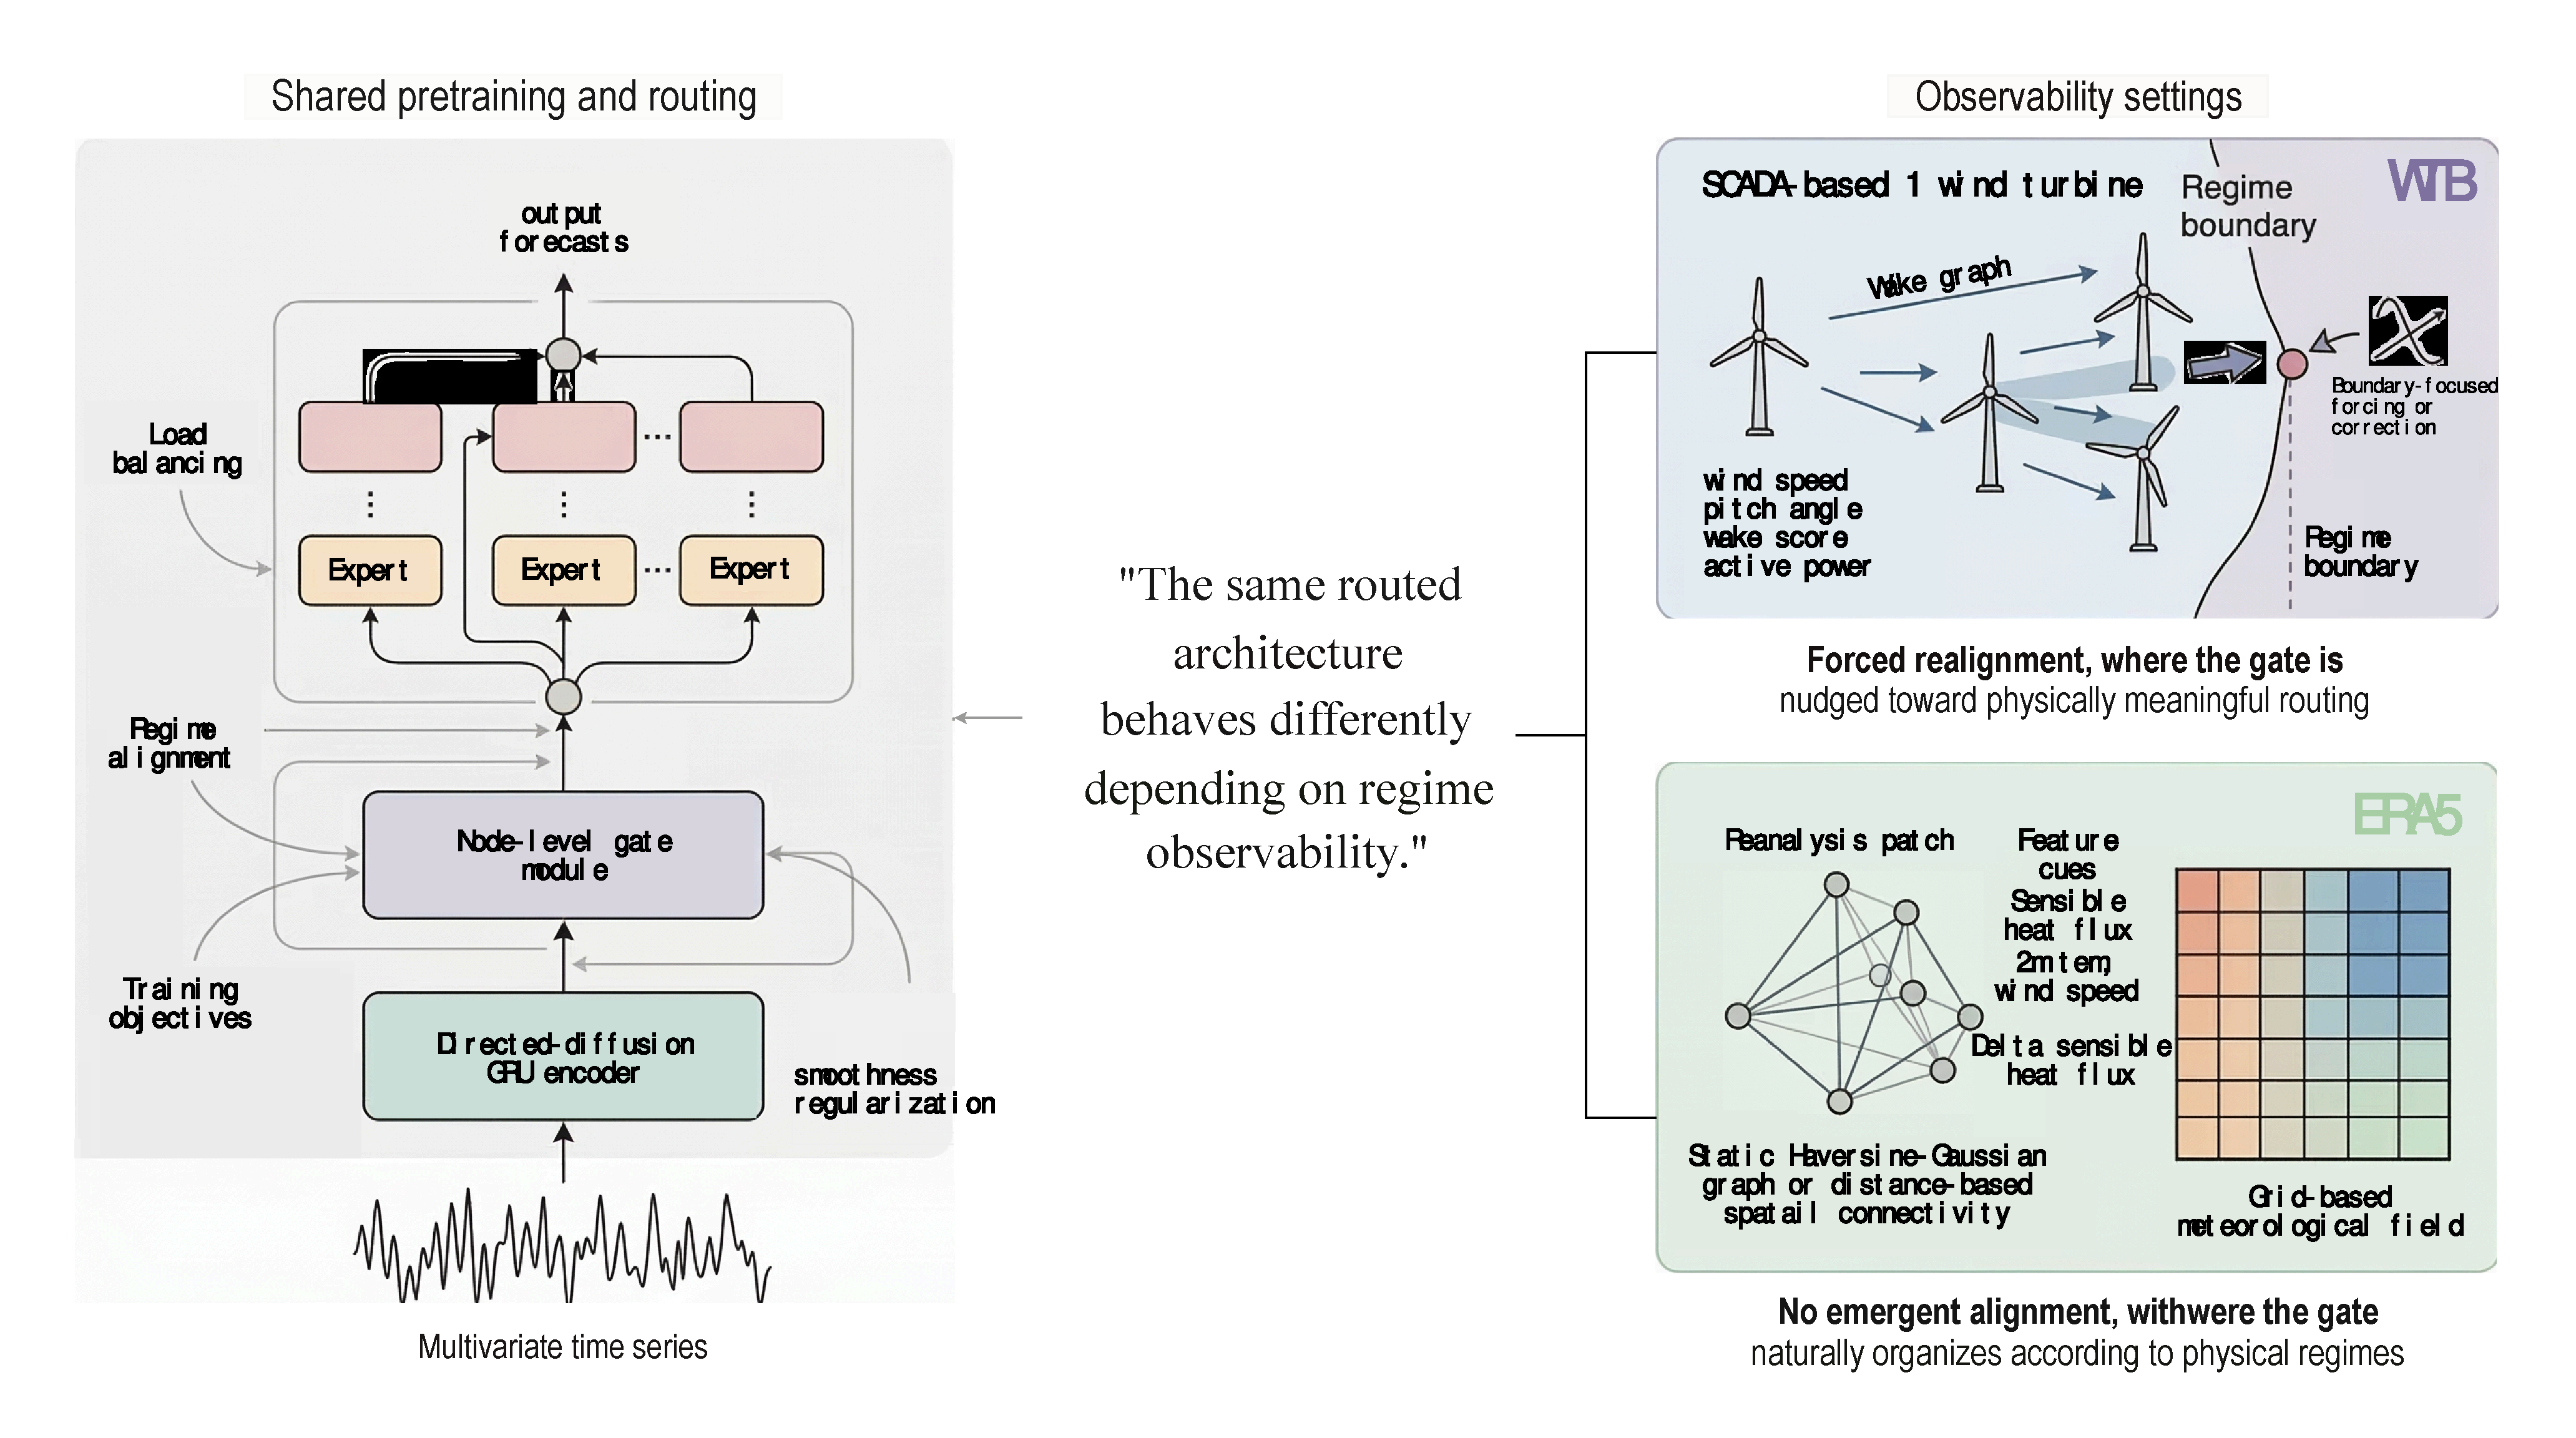
\includegraphics[width=0.95\linewidth,height=\textheight,keepaspectratio,alt={Physics-aligned regime-aware MoE. The two datasets share the same directed-diffusion GRU encoder and node-level MoE routing mechanism. WTB uses a dynamic wake graph and a boundary-focused forcing term, whereas ERA5 uses a Haversine-Gaussian graph and a thermodynamic regime anchor.}]{artifacts/final_evidence_package/export/figures/figure1_architecture.pdf}
\caption{Physics-aligned regime-aware MoE. The two datasets share the
same directed-diffusion GRU encoder and node-level MoE routing
mechanism. WTB uses a dynamic wake graph and a boundary-focused forcing
term, whereas ERA5 uses a Haversine-Gaussian graph and a thermodynamic
regime anchor.}
\end{figure}

\subsection{Integration of Physical Constraints into Model
Optimization}\label{integration-of-physical-constraints-into-model-optimization}

Prediction loss does not uniquely identify the gate when several experts
can fit averaged dynamics similarly well
{[}\citeproc{ref-shazeer2017outrageously}{8},\citeproc{ref-fedus2022switch}{9}{]}.
WTB makes this failure visible: inflow variation, wake disturbance, and
pitch control are observed together, so a low-loss router can still
ignore the operating boundary. We use routing regularizers for the
specific failure modes that matter here. The total objective is

\[
\mathcal{L}
=
\mathcal{L}_{\mathrm{pred}}
+
\lambda_{\mathrm{bal}}\mathcal{L}_{\mathrm{bal}}
+
\lambda_{\mathrm{align}}\mathcal{L}_{\mathrm{align}}
+
\lambda_{\mathrm{force}}\mathcal{L}_{\mathrm{force}}
+
\lambda_{\mathrm{aux}}\mathcal{L}_{\mathrm{aux}}
+
\lambda_{\mathrm{smooth}}\mathcal{L}_{\mathrm{smooth}},
\]

with inactive terms set to zero. Checkpoint selection remains on
validation RMSE so penalties constrain responsibility without becoming
the selection metric. Exact weights are in Appendix A.

\subsubsection{Load balancing}\label{load-balancing}

A balancing term prevents early expert collapse before regime-specific
structure has time to emerge. It couples hard top-\(K\) usage with soft
probability mass over valid node-time samples. Appendix A gives the
exact expression; physical ownership is supplied only by the anchored
alignment terms below.

\subsubsection{Regime-anchor alignment}\label{regime-anchor-alignment}

The alignment term connects the first \(C\) gate logits to the declared
regime structure so that cross-seed statements such as ``MPPT-aligned''
refer to a fixed mapping rather than to post-hoc relabeling. With
\(\mathbf{z}^{(1:C)}_{i,t}\) denoting the anchored logits, \(R_{i,t}\)
the label, and \(M_{i,t}\) the validity mask, \[
\begin{aligned}
\mathcal{L}_{\mathrm{align}}
&= \frac{1}{|\Omega|}
\sum_{(i,t)\in\Omega}
\mathrm{CE}\!\left(\mathbf{z}^{(1:C)}_{i,t}, R_{i,t}\right),\\
\Omega&=\{(i,t):M_{i,t}=1\}.
\end{aligned}
\] with inverse-frequency class weights on the training split.

\subsubsection{Boundary-focused forcing (WTB
only)}\label{boundary-focused-forcing-wtb-only}

After coarse alignment the boundary remains partly masked by control
action. A focused forcing term acts on MPPT and pitch-control samples
only. With
\(Y^{\mathrm{force}}_{i,t}=\mathbf{1}[R^{\mathrm{wtb}}_{i,t}=2]\) for
\(R^{\mathrm{wtb}}_{i,t}\in\{1,2\}\),
\[\mathcal{L}_{\mathrm{force}} = \frac{1}{|\Omega_{\mathrm{force}}|}\sum_{(i,t)\in\Omega_{\mathrm{force}}}\mathrm{CE}\!\left(\left[z^{(\mathrm{mppt})}_{i,t}, z^{(\mathrm{pitch})}_{i,t}\right]^{\top}, Y^{\mathrm{force}}_{i,t}\right),\]
where
\(\Omega_{\mathrm{force}}=\{(i,t):R^{\mathrm{wtb}}_{i,t}\in\{1,2\}, M_{i,t}=1\}\).
This term is not a lead-time switch predictor; it is a boundary
identifiability regularizer for the issue-time operating state.

\subsubsection{Wake auxiliary supervision and graph
smoothness}\label{wake-auxiliary-supervision-and-graph-smoothness}

A wake auxiliary label identifies residual wake ambiguity inside MPPT
and pitch-control samples, and a graph-smoothness penalty discourages
noisy neighbor-to-neighbor gate jumps. Both formulas are in Appendix A.

\subsection{Operational reserve diagnostic
protocol}\label{operational-reserve-diagnostic-protocol}

The reserve diagnostic tests whether a physically auditable gate changes
the reserve tradeoff in the MPPT-to-pitch window after the
point-forecast model has been trained. For each saved WTB run,
validation predictions select reserve levels; test predictions are then
evaluated once with those levels fixed. The protocol follows the same
information boundary as an operator who calibrates a short-term reserve
rule before using it on a later period.

Let \(\hat{y}_{i,t}\) be the scheduled point forecast and \(y_{i,t}\)
the realized active power at an evaluated horizon cell. We define
over-forecast shortfall as

\[
s_{i,t} = \max(\hat{y}_{i,t} - y_{i,t}, 0),
\]

because this is the error direction that leaves a reserve schedule
exposed. For a reserve policy \(b\) and empirical quantile \(q\), the
validation split estimates a reserve level

\[
r_{b,q} = Q_q\!\left(\{s_{i,t}: (i,t)\in b,\ (i,t)\in \mathcal{V}\}\right),
\]

where \(Q_q\) is an empirical quantile and \(\mathcal{V}\) is the
validation split. The grid is fixed before test evaluation:

\[
q \in \{0.50,0.60,0.70,0.80,0.85,0.90,0.95,0.975,0.99\}.
\]

The reserve bin \(b\) is either the whole sample, a physical operating
bin, or a gate-derived bin. For each shortage-to-reserve cost ratio
\(\rho\), the protocol selects the validation quantile that minimizes

\[
C_{\mathcal{V}}(b,q;\rho)
=
\sum_{(i,t)\in b\cap \mathcal{V}}
\left[
r_{b,q} + \rho \max(s_{i,t}-r_{b,q},0)
\right]\Delta t.
\]

The selected \((b,q)\) rule is then frozen and applied to the test
split. The reported test metrics are total cost \(C\), violation rate
\(\Pr[s_{i,t}>r_b]\), reserve energy \(\sum r_b\Delta t\), and shortage
energy \(\sum \max(s_{i,t}-r_b,0)\Delta t\). All totals are reported in
normalized reserve-energy cost units. Thus a value written as 84.58M
denotes 84.58 million normalized reserve-energy cost units, not
currency.

The cost ratio \(\rho\) is an energy-system assumption rather than an
abstract tuning knob. If the marginal cost of carrying one unit of
reserve energy is \(C_r\), then \(\rho=10\) charges one unit of residual
shortage as \(10C_r\). Ratios 5--10 represent moderate reliability
settings such as transition-window scheduling or imbalance screening;
ratios 20--50 represent scarcity-aware screening where shortage
avoidance dominates local cost savings. The primary diagnostic compares
Graph WaveNet/global, Graph WaveNet/physical-bin, boundary
router/global, and boundary router/gate-bin policies. Only same-model
global comparisons attribute gate-bin reserve effects to the learned
router.

To bound this diagnostic against a probabilistic reserve alternative, we
additionally run validation-frozen empirical quantile baselines for the
global and physical operating bins. These are not trained distributional
forecasters; they are conformal-style shortfall reserves estimated on
the validation split and evaluated once on the test split. The main
reported boundary window is fixed at \(\pm 1.0\) m s\(^{-1}\) around
rated wind and the main cost ratio is \(\rho=10\), with sensitivity at
\(\rho \in \{2,5,10,20,50\}\). A separate toy operational-cost module
reports the same normalized decision as reserve procurement cost plus
\(\rho\)-weighted residual-shortage penalty. It deliberately excludes
optimal power flow, unit commitment, market clearing, delivery
constraints, and price claims.

\begingroup
\footnotesize
\setlength{\fboxsep}{5pt}
\noindent\fbox{\begin{minipage}{0.96\linewidth}
\textbf{Reserve diagnostic algorithm.}
Input saved validation/test point forecasts, targets, masks, physical anchors, and gate outputs.
Compute over-forecast shortfall on valid cells.
Form global, physical-bin, and gate-bin reserve groups on validation outputs only.
For each cost ratio and group, select the empirical shortfall quantile that minimizes validation reserve-plus-shortage cost.
Freeze the selected reserve levels and evaluate them once on test cells.
Aggregate cost, violation rate, reserve energy, and shortage energy over full, boundary, transition, ramp, horizon-bucket, and time-of-day slices.
Report horizon-specific empirical-quantile rows only as a post-hoc what-if.
Compare validation-frozen global and physical-bin quantile reserves as bounded probabilistic baselines.
Report toy operating cost only as reserve procurement plus shortage penalty, not as dispatch.
\end{minipage}}
\par
\endgroup

\section{Case Study Configuration and Operational
Constraints}\label{case-study-configuration-and-operational-constraints}

\subsection{Datasets and
preprocessing}\label{datasets-and-preprocessing}

The experiment uses two observability settings, not two interchangeable
benchmarks. WTB is the control-confounded case. The KDD Cup 2022
benchmark contains 134 turbines and 245 days of 10 min SCADA
measurements {[}\citeproc{ref-zhou2024sdwpfdata}{19}{]}. The
MPPT-to-pitch transition is only indirectly visible because inflow
variation, wake disturbance, and blade-pitch control are mixed in the
same stream.

The data are reorganized into synchronous tensors with \(T=35{,}280\)
time steps, \(N=134\) turbines, and \(F=11\) dynamic inputs. Missing
inputs are forward-filled within turbine and then completed with
training-set means. Invalid or non-positive active power is retained
only through its mask so that the model still sees operational
irregularity without treating those points as supervised targets.

ERA5 is the signal-expressive case. We use three archived months over a
fixed \(16 \times 16\) hourly patch
{[}\citeproc{ref-hersbach2020era5}{24}{]}. Sensible heat flux and its
temporal variation make the stable-to-convective transition directly
observable. The retained tensor has \(T=2208\) frames, \(N=256\) nodes,
and eight input variables. Both datasets use the same history and
horizon lengths, \(H=36\) and \(P=24\), so differences in performance
cannot be attributed to unequal context length. The chronological split
is 180/30/35 days for WTB and 1325/441/442 frames for ERA5.

\subsection{Techno-Economic Validation and Benchmarking
Framework}\label{techno-economic-validation-and-benchmarking-framework}

The comparison has two layers. The first isolates the routing mechanism
after shared-capacity explanations have been controlled. The dense
baseline uses the same directed-diffusion GRU encoder and replaces the
expert mixture with one dense prediction head. The unconstrained MoE
adds routed capacity without physical correction. The corrected-routing
comparator is dataset-specific: ERA5 uses the full corrected stack,
while WTB uses the boundary-focused variant selected for gate recovery.
Parameter budgets are matched in WTB and near-matched in ERA5, where the
dense model has 103,272 parameters and the routed models have 103,843
parameters.

The second layer tests the RMSE price against stronger and more
engineering-facing baselines. Graph WaveNet, Graph Transformer, GAT-GRU,
and PatchTST are included for WTB, together with deterministic
persistence, a fitted physical power-curve baseline, XGBoost and
LightGBM lag-feature predictors, and a DLinear-style LTSF baseline.
Graph WaveNet, STGCN, PatchTST, TCN, and a deterministic persistence
predictor are included for ERA5. This split avoids using one comparison
for two different claims. The in-family layer tests whether physical
routing changes the learned partition under a fixed backbone. The
baseline layer tests whether the routing intervention remains honest
about forecast error when compared with established temporal, graph, and
engineering predictors.

For compactness, the mechanism tables shorten the three in-family model
names to \textbf{Dense (matched)}, \textbf{Unconstrained MoE}, and
\textbf{Corrected routing comparator}. The WTB forecasting tables
additionally report Graph WaveNet, Graph Transformer, GAT-GRU, PatchTST,
the full physics-aligned MoE, the WTB boundary-forced router, and
engineering baselines built from persistence, power curves,
gradient-boosted lag features, and a DLinear-style LTSF readout. The
ERA5 forecasting tables additionally report persistence and four learned
external baselines. The in-family mechanism families are summarized in
Appendix A so that the Results section can focus on evidence rather than
model bookkeeping.

\subsection{Training protocol and evaluation
metrics}\label{training-protocol-and-evaluation-metrics}

All neural models use the same training protocol where the architecture
permits it. We use AdamW, early stopping on validation RMSE, gradient
clipping, and mixed-precision training on a single CUDA-enabled GPU.
Exact optimizer constants are reported in the Appendix so that the main
text can stay focused on the comparison logic. The WTB dense baseline,
Unconstrained MoE, full physics-aligned MoE, and boundary-forced router
are repeated across five strict-mask seeds. The synchronized
strong-baseline refresh covers Graph WaveNet, Graph Transformer,
GAT-GRU, and PatchTST across seeds 201--205, giving 20 completed
baseline runs under the same strict anchor-valid evaluation cache. The
engineering WTB baselines are deterministic or sampled single-run
readouts from the same frozen cache and are used to anchor practical
forecast difficulty rather than to make a seed-level neural ranking.
ERA5 main in-family models are repeated across five seeds, and the ERA5
learned baselines are repeated across three seeds. Thresholds and
routing weights are set before test evaluation and then audited by
sensitivity sweeps and boundary negative controls, so the main routing
result is not selected by test-set NMI.

The metrics follow the claim. Overall MAE and RMSE measure forecasting
accuracy. Switch-window MAE and RMSE use the evaluator's
transition-window mask around regime changes. This is distinct from the
later boundary-band audit, which isolates anchors within +/-1.0 m
s\(^{-1}\) of the WTB rated-wind MPPT-to-pitch boundary. Regime-wise
RMSE locates the error reduction. Normalized mutual information (NMI),
adjusted Rand index (ARI), usage entropy, and confusion matrices test
whether the gate corresponds to physically interpretable structure.

Figure 2 gives the operating-decision context before the forecasting
results are introduced: graph geometry shows where forecast errors
propagate, and the regime-anchor panels show which sensor-derived
boundaries can support reserve diagnostics.

\begin{figure}
\centering
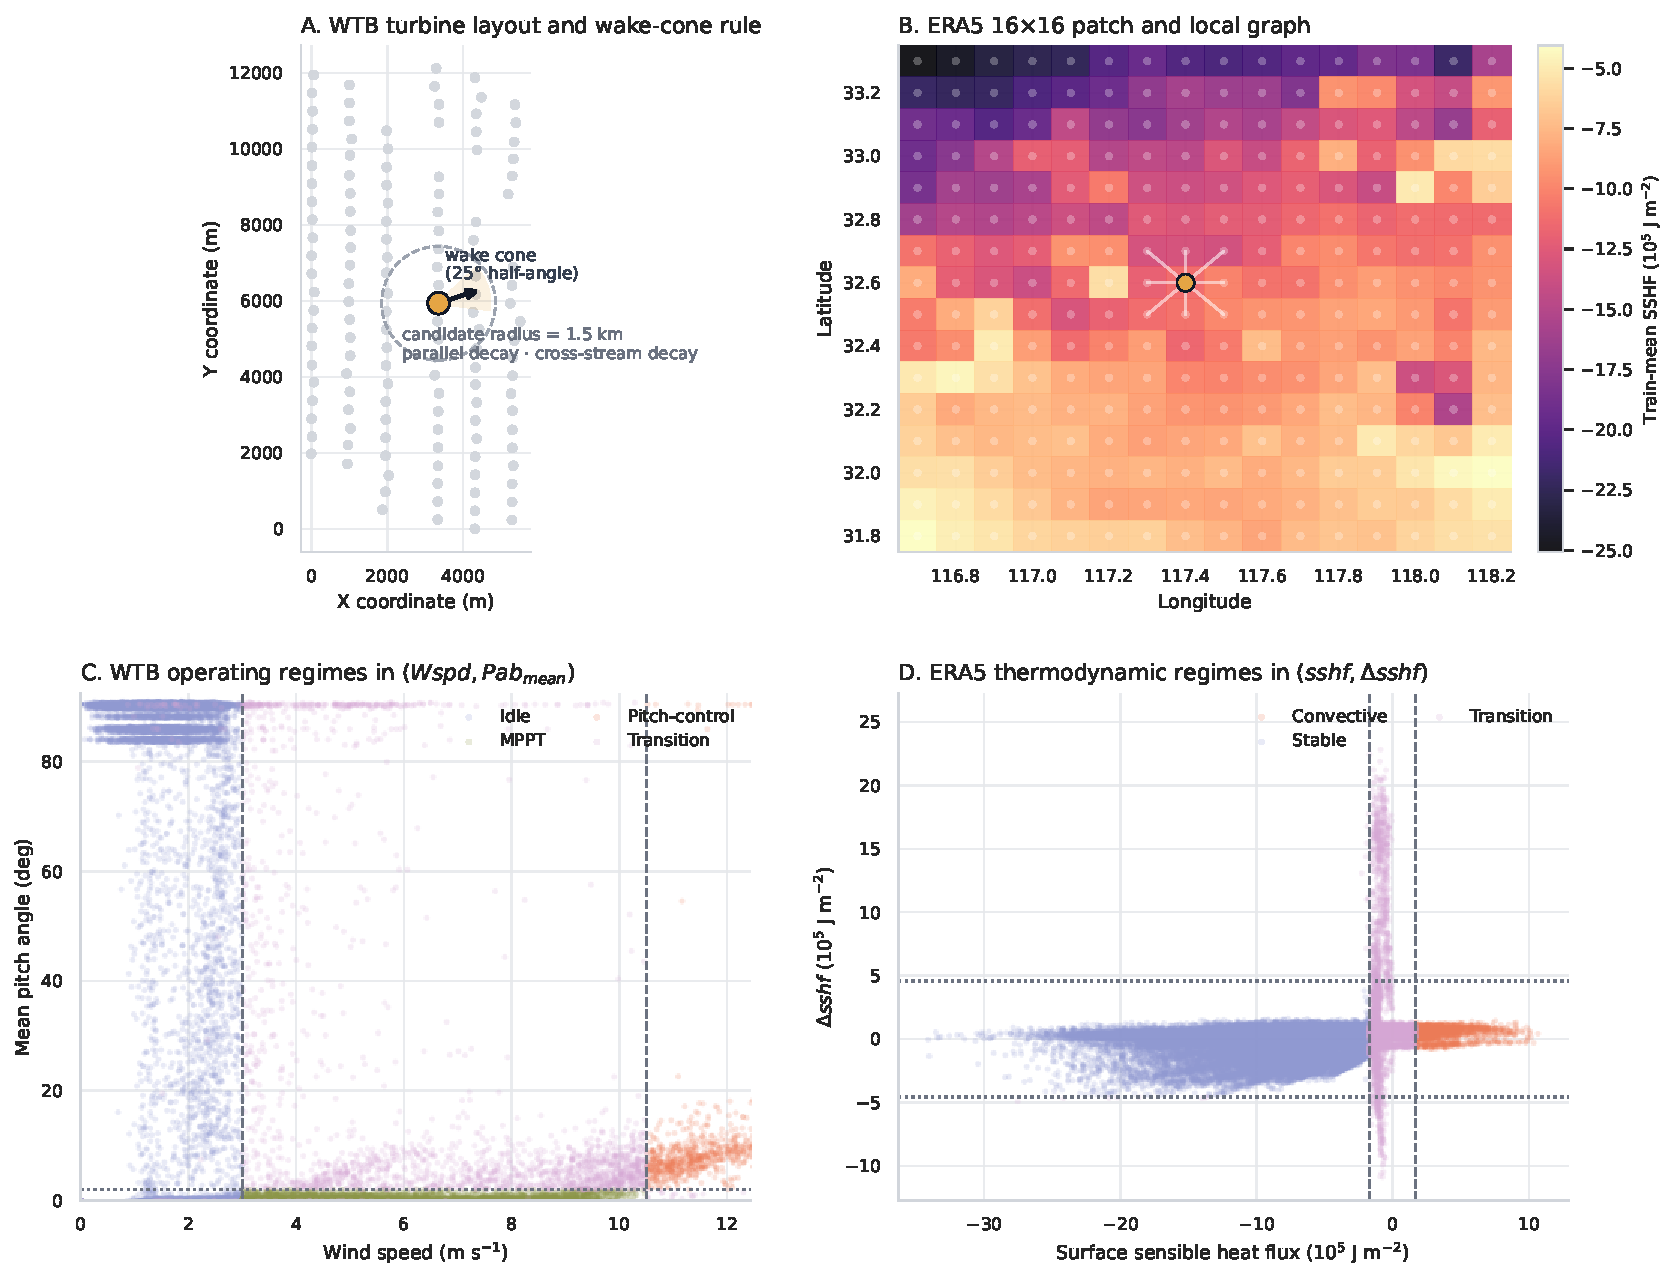
\includegraphics[width=0.97\linewidth,height=\textheight,keepaspectratio,alt={Operating-decision context and physical regime anchors. (A) WTB turbine layout with the schematic wake cone and retained candidate radius used in the dynamic directed wake graph. (B) ERA5 16x16 patch with training-mean sensible heat flux and local Haversine-Gaussian graph connections around the central node. (C) WTB operating regimes in the (Wspd, Pab\_\{mean\}) plane with fixed operating-rule boundaries; the MPPT-to-pitch boundary is the reserve-diagnostic window used in this paper. (D) ERA5 thermodynamic regimes in the (sshf, \textbackslash Delta sshf) plane with thresholds estimated from the training split, included as an observability contrast.}]{artifacts/final_evidence_package/export/figures/figure2_data_boundary.pdf}
\caption{Operating-decision context and physical regime anchors. (A) WTB
turbine layout with the schematic wake cone and retained candidate
radius used in the dynamic directed wake graph. (B) ERA5 16x16 patch
with training-mean sensible heat flux and local Haversine-Gaussian graph
connections around the central node. (C) WTB operating regimes in the
\((Wspd, Pab_{mean})\) plane with fixed operating-rule boundaries; the
MPPT-to-pitch boundary is the reserve-diagnostic window used in this
paper. (D) ERA5 thermodynamic regimes in the \((sshf, \Delta sshf)\)
plane with thresholds estimated from the training split, included as an
observability contrast.}
\end{figure}

\section{Evidence and Operational Boundary
Diagnosis}\label{evidence-and-operational-boundary-diagnosis}

The results answer three operational questions rather than following the
order in which experiments were run. First, can a routed forecaster
recover a physically declared operating boundary and retain value when
the corresponding threshold labels degrade? Second, does that auditable
gate change the reserve tradeoff in the MPPT-to-pitch window? Third,
what accuracy price and deployment gate determine whether the diagnostic
should be used at a new wind farm?

\subsection{Can the Gate Recover the Operating
Boundary?}\label{can-the-gate-recover-the-operating-boundary}

SCADA-anchored routing recovers the WTB MPPT-to-pitch partition strongly
enough to make the gate an auditable operating-boundary signal. Across
five WTB seeds, the boundary-forced router reaches NMI about 0.87 and
ARI about 0.92 against the declared MPPT-to-pitch labels. This is not
the lowest-RMSE forecaster in the benchmark; Graph WaveNet reaches
overall RMSE 225.74 +/- 2.60, while the boundary-forced router reaches
236.13 +/- 8.41. The point of the comparison is therefore not accuracy
dominance. The strong baseline sets the forecasting price paid to obtain
a physically traceable responsibility assignment.

The boundary itself is a meaningful diagnostic target. Anchors within
+/-1.0 m s\(^{-1}\) of rated wind have RMSE 321.17 +/- 21.31, roughly 67
units above valid non-boundary MPPT/pitch anchors. The same boundary
band has mixed-regime structure (NMI/ARI 0.6562/0.7766), so it is both a
forecasting stress point and a natural reserve-risk window. ERA5
provides the positive observability contrast: when the regime marker is
directly visible through sensible heat flux, routing correction improves
alignment without changing the headline accuracy story.

\begin{table}[H]
\centering
\footnotesize
\setlength{\tabcolsep}{4pt}
\renewcommand{\arraystretch}{1.08}
\caption{Operating-boundary recovery and mechanism checks.}
\begin{tabularx}{0.98\linewidth}{>{\raggedright\arraybackslash}p{0.30\linewidth} >{\raggedright\arraybackslash}p{0.34\linewidth} >{\raggedright\arraybackslash}X}
\toprule
Check & Metric & Result \\
\midrule
WTB boundary-forced router & Gate-regime NMI / ARI & 0.8716 +/- 0.0418 / 0.9166 +/- 0.0371 \\
WTB boundary-band audit & Boundary-band RMSE; mixed-regime NMI / ARI & 321.17 +/- 21.31; 0.6562 / 0.7766 \\
Boundary-anchor intervention & Overall RMSE change; NMI / ARI drop & +2.6792; 0.7017 / 0.8593 \\
WTB spatial and time holdouts & Held-out-node NMI / ARI; future-holdout NMI / ARI & 0.8340 / 0.8829; 0.8352 / 0.8870 \\
Threshold-grid audit & Worst-case saved-gate NMI / ARI & 0.8655 +/- 0.0429 / 0.9146 +/- 0.0377 \\
\bottomrule
\end{tabularx}
\end{table}

The diagnostic survives the main falsification checks. Zeroing the
intended boundary anchor sharply reduces gate-regime agreement, whereas
zeroing the wake score is near-null. Placebo labels do not reproduce the
actual-label agreement. Spatial holdout, future-period holdout, and
threshold sweeps preserve routing semantics.

The gate also provides value that a threshold label stream cannot
provide when that stream degrades. We audit saved five-seed gates around
MPPT-to-pitch transitions after delaying the threshold labels, randomly
dropping label availability, and recomputing threshold labels under
sensor noise. Table\textasciitilde{}\ref{tab:early-warning} reports
recall on early pitch-control cells in a six-step transition window.
With a six-step label delay, the delayed threshold rule recalls only
0.196 of early pitch cells, whereas the gate recalls 0.960. With 50\%
label availability, the available-label rule recalls 0.508, while the
gate remains at 0.960. Under the strongest sensor-noise setting tested,
the threshold rule drops to 0.652 recall and the gate remains unchanged
because the saved gate is evaluated as an already issued diagnostic
signal. This is the operational meaning of auditability in the paper:
the gate is not merely reproducing a perfect contemporaneous threshold
label, but preserving a transition-window diagnostic when that label is
delayed, incomplete, or noisy.

We price this accountability explicitly. A model receives citable
degraded-label gain only after its route passes the physical-routing
audit; otherwise the accountability gain is set to zero, even for an
accurate or routed-capacity model. Under this rule Graph WaveNet is the
zero-RMSE-price anchor without an audited operating-state route,
Unconstrained MoE fails the route audit (NMI 0.014), and the
boundary-forced router is the only current point that exchanges a
10.39-RMSE price for +0.764 six-step-delay recall gain, recovering about
566 early pitch-window cells per seed relative to the delayed threshold
rule (Fig.\textasciitilde{}\ref{fig:accountability-tradeoff}).

\begin{table}[H]
\centering
\scriptsize
\setlength{\tabcolsep}{1.5pt}
\renewcommand{\arraystretch}{1.05}
\caption{Label-degradation audit for early MPPT-to-pitch pitch-window detection.}
\label{tab:early-warning}
\begin{tabularx}{0.98\linewidth}{>{\raggedright\arraybackslash}p{0.24\linewidth} >{\raggedright\arraybackslash}p{0.24\linewidth} >{\centering\arraybackslash}p{0.13\linewidth} >{\centering\arraybackslash}p{0.13\linewidth} >{\centering\arraybackslash}X}
\toprule
Scenario & Setting & Gate & Rule & Gain \\
\midrule
Delay & 1 step & 0.960 & 0.655 & +0.305 \\
Delay & 3 steps & 0.960 & 0.381 & +0.579 \\
Delay & 6 steps & 0.960 & 0.196 & +0.764 \\
Availability & 75\% labels & 0.960 & 0.744 & +0.216 \\
Availability & 50\% labels & 0.960 & 0.508 & +0.452 \\
Availability & 25\% labels & 0.960 & 0.242 & +0.718 \\
Noise & Wspd 0.5, Pab 1.0 & 0.960 & 0.808 & +0.152 \\
Noise & Wspd 1.0, Pab 2.0 & 0.960 & 0.652 & +0.308 \\
\bottomrule
\end{tabularx}
\end{table}

\begin{table}[H]
\centering
\tiny
\setlength{\tabcolsep}{1pt}
\renewcommand{\arraystretch}{1.08}
\caption{Anchor-observability stress: 245d WTB test NMI/ARI.}
\begin{tabularx}{0.98\linewidth}{>{\raggedright\arraybackslash}p{0.18\linewidth} >{\centering\arraybackslash}p{0.115\linewidth} >{\centering\arraybackslash}p{0.115\linewidth} >{\centering\arraybackslash}p{0.115\linewidth} >{\centering\arraybackslash}p{0.115\linewidth} >{\centering\arraybackslash}p{0.115\linewidth} >{\centering\arraybackslash}X}
\toprule
Variant & 201 & 202 & 203 & 204 & 205 & Mean \\
\midrule
no Patv & .878/.928 & .966/.985 & .703/.719 & .914/.954 & .945/.973 & .881 \\
no Pab\_mean & .880/.932 & .906/.947 & .889/.937 & .923/.961 & .792/.865 & .878 \\
lag Patv & .475/.390 & .899/.935 & .734/.765 & .741/.769 & .965/.984 & .763 \\
lag Pab/Wspd & .398/.299 & .755/.814 & .699/.766 & .784/.864 & .784/.858 & .684 \\
\bottomrule
\end{tabularx}
\end{table}

The training-level anchor-stress guard has been completed across five
seeds. Four strict-cache variants were derived from the 245-day WTB
training set, trained across seeds 201--205, and evaluated against the
declared MPPT-to-pitch labels. The table reports the test-set NMI/ARI
scores. Removing \texttt{Patv} or \texttt{Pab\_mean} individually leaves
the gate essentially intact (mean 0.881 and 0.878, respectively).
Lagging \texttt{Patv} lowers one seed but the five-seed mean remains
above the 0.65 threshold (0.763). Lagging both \texttt{Pab\_mean} and
\texttt{Wspd} also lowers one seed, yet the five-seed mean crosses the
threshold (0.684). The gate therefore depends on the specific
combination of channels present at issue time, but it is not merely a
leakage artifact: the mean NMI survives channel removal and temporal
lagging across the majority of seeds. The manuscript uses the wording
``partial anchor robustness'' rather than ``anchor-free physical
discovery.'' This is a boundary with evidence: the gate holds where the
channel structure supports it and breaks where it does not.

\begin{table}[H]
\centering
\footnotesize
\setlength{\tabcolsep}{5pt}
\renewcommand{\arraystretch}{1.08}
\caption{Training-level anchor-stress guard for claim control (five-seed update).}
\begin{tabularx}{0.98\linewidth}{>{\raggedright\arraybackslash}p{0.31\linewidth} >{\raggedright\arraybackslash}p{0.35\linewidth} >{\raggedright\arraybackslash}X}
\toprule
Stress component & Guard status & Manuscript consequence \\
\midrule
Strict-cache variants & no-\texttt{Patv}, lagged-\texttt{Patv}, no-\texttt{Pab\_mean}, lagged pitch/wind-speed caches derived & Anchor observability is explicitly testable \\
Leakage guard & Cache-level guard passed; all 20 training runs completed & No leakage warning from derived variants \\
Five-seed NMI gate & no-\texttt{Patv} (0.881), no-\texttt{Pab\_mean} (0.878), lagged-\texttt{Patv} (0.763), lagged pitch/wind-speed (0.684); all cross 0.65 & Partial anchor robustness supported across all variants \\
Claim boundary & All 5-seed means cross 0.65; gate holds under single-anchor removal and dual-channel lagging & Use ``partial anchor robustness'' language, not anchor-free discovery \\
\bottomrule
\end{tabularx}
\end{table}

\begin{figure}
\centering
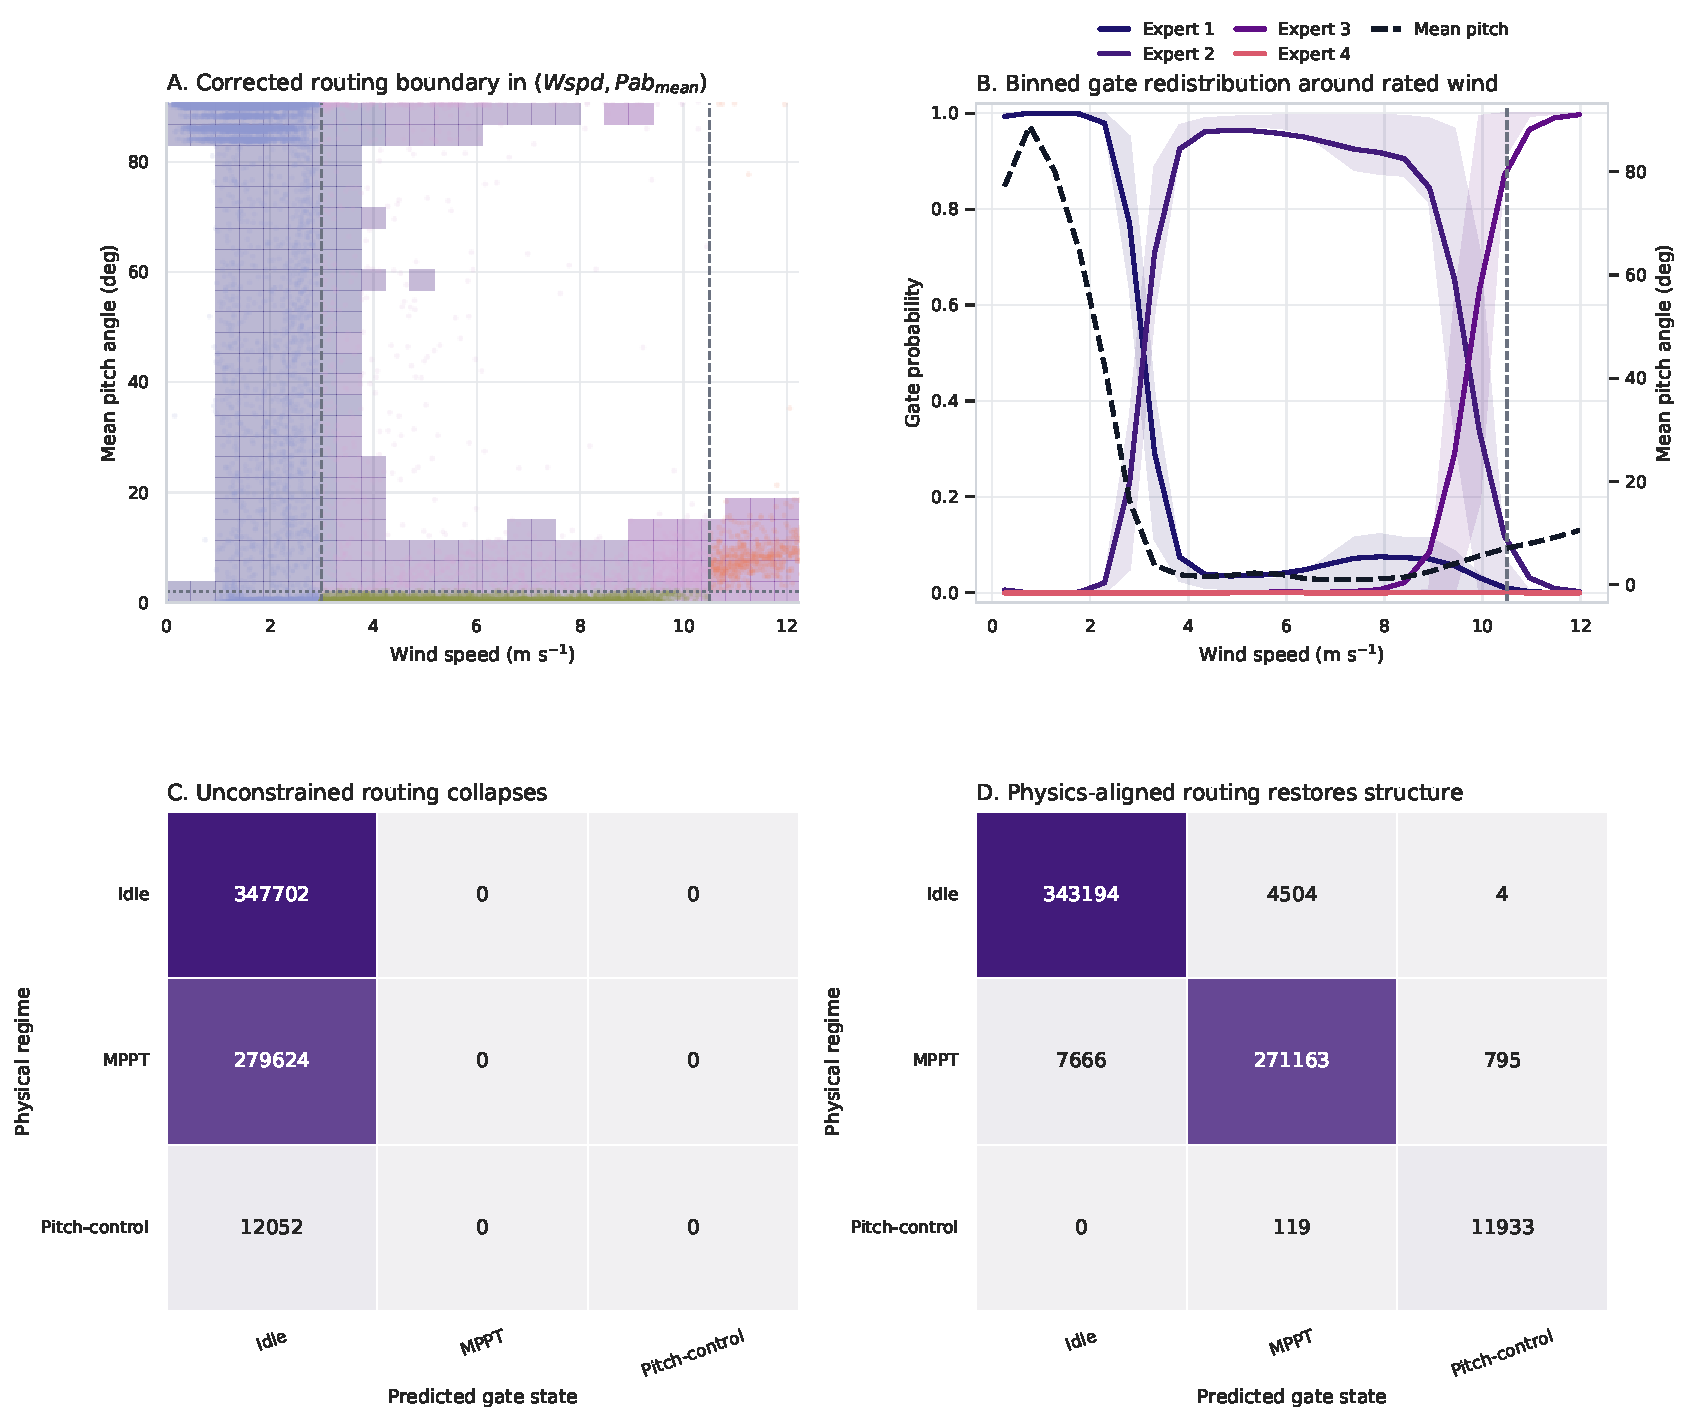
\includegraphics[width=0.97\linewidth,height=\textheight,keepaspectratio,alt={The WTB operating plane shows the main mechanism: after correction, the dominant routed responsibility changes around the rated-wind and pitch-control boundary instead of forming an arbitrary expert partition. The confusion matrices summarize the same recovery numerically.}]{artifacts/final_evidence_package/export/figures/figure4_routing_evidence.pdf}
\caption{The WTB operating plane shows the main mechanism: after
correction, the dominant routed responsibility changes around the
rated-wind and pitch-control boundary instead of forming an arbitrary
expert partition. The confusion matrices summarize the same recovery
numerically.}
\end{figure}

\begin{figure}
\centering
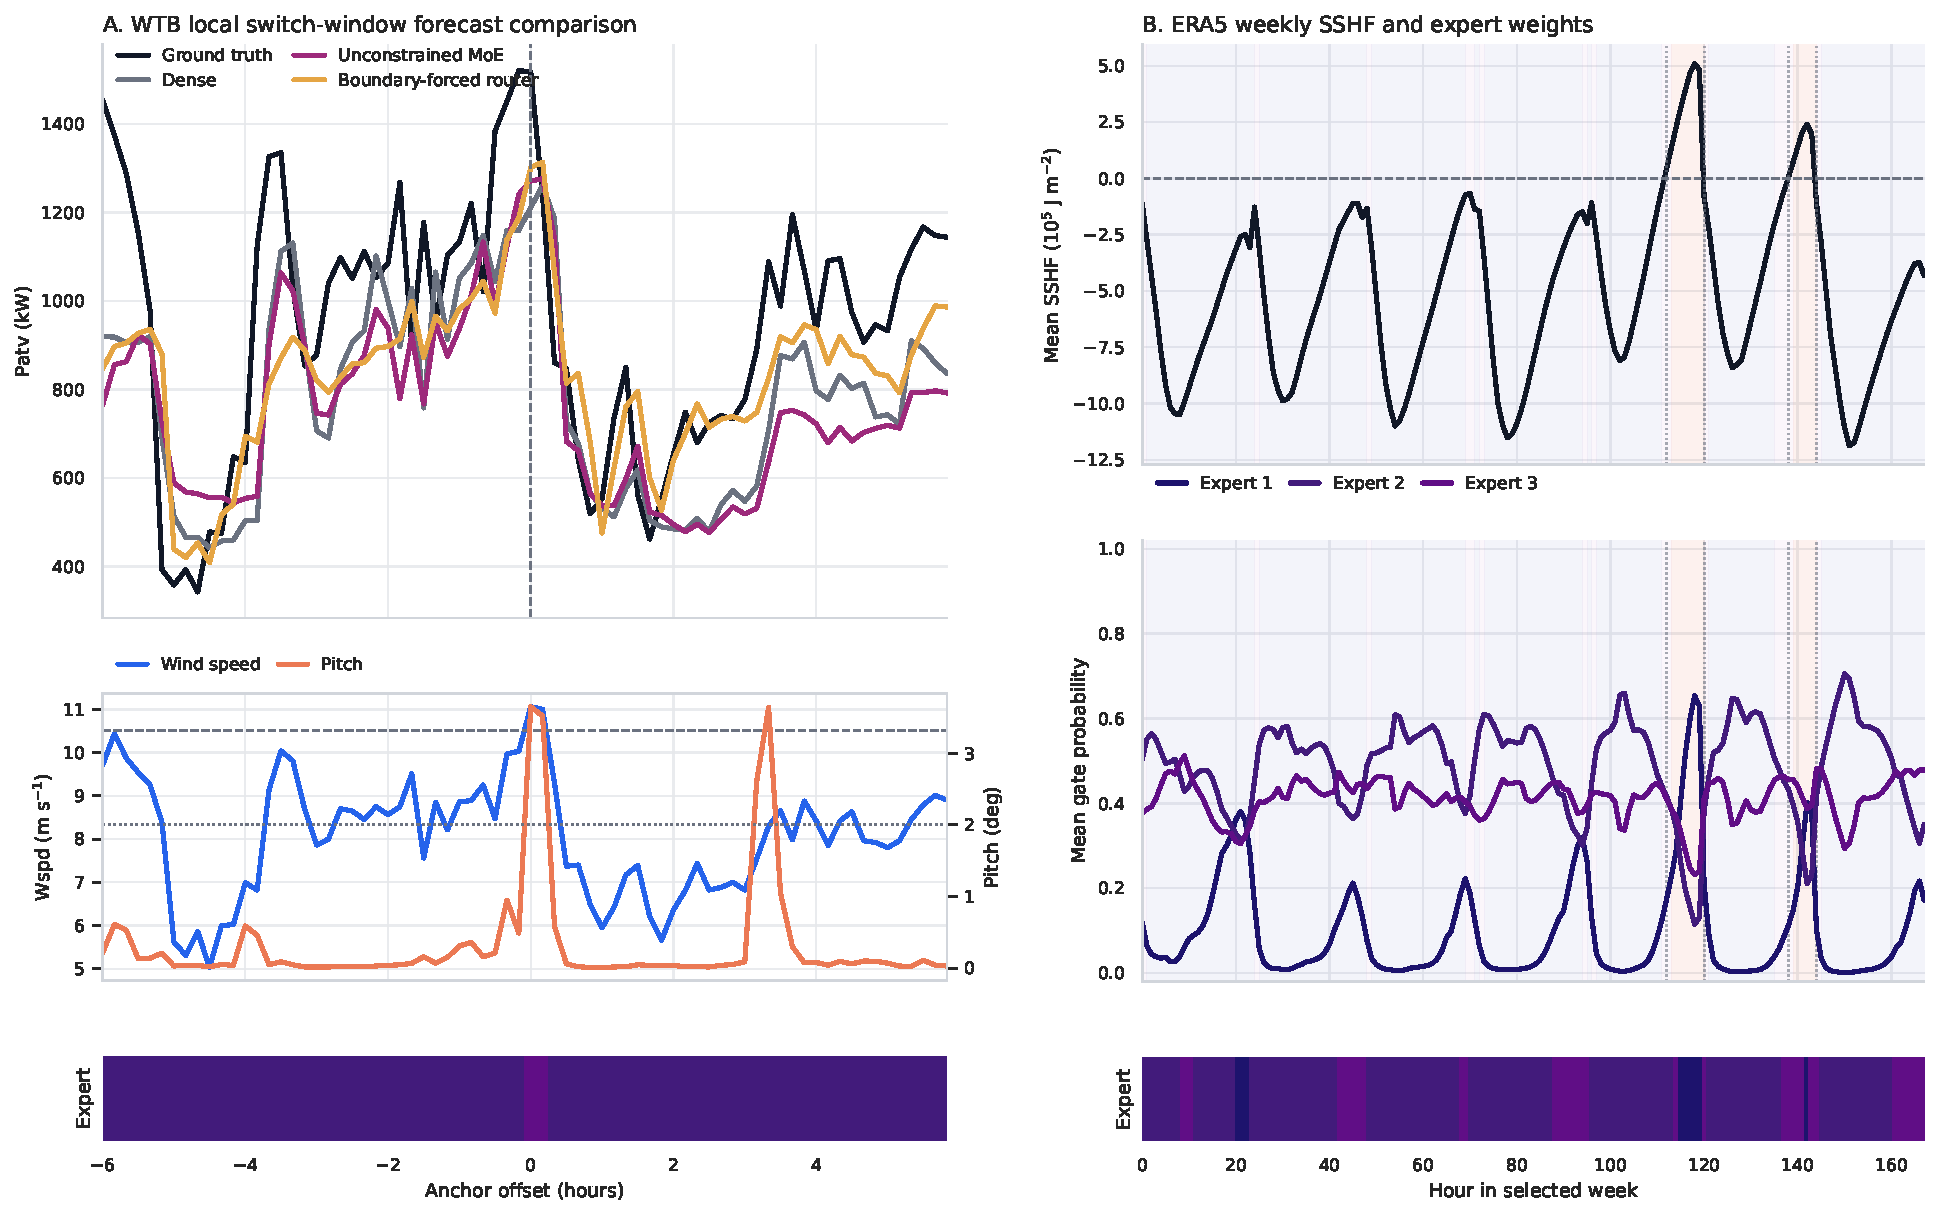
\includegraphics[width=0.97\linewidth,height=\textheight,keepaspectratio,alt={The time-series case studies show why observability matters. The WTB gate tracks a turbine-control switch that is partly hidden inside SCADA control action, whereas the ERA5 gate follows a more directly observed thermodynamic marker.}]{artifacts/final_evidence_package/export/figures/figure5_case_studies.pdf}
\caption{The time-series case studies show why observability matters.
The WTB gate tracks a turbine-control switch that is partly hidden
inside SCADA control action, whereas the ERA5 gate follows a more
directly observed thermodynamic marker.}
\end{figure}

\subsection{Boundary-Risk Vignette: Does the Gate Change Reserve
Tradeoffs?}\label{boundary-risk-vignette-does-the-gate-change-reserve-tradeoffs}

The reserve audit asks whether a recovered physical gate changes the
reserve tradeoff in the operating window where over-forecasts become
unmet reserve requirements. Four policies separate the effects: Graph
WaveNet/global (low-RMSE reference), Graph WaveNet/physical-bin
(physical stratification without learned gate), Boundary router/global
(routed model with single reserve rule), and Boundary router/gate-bin
(gate-conditioned allocation on the same routed predictor).

At shortage-to-reserve cost ratio 10, gate-conditioned binning exchanges
about 3.6\% additional reserve energy for a 14.5\% reduction in shortage
energy and a 1.38 percentage-point reduction in boundary-window
violation relative to the same routed model with a global rule. The
comparison is deliberately same-model: the reserve change is attributed
to gate-conditioned allocation, not to a different forecasting backbone.

The validation-frozen quantile baseline changes how the result should be
read. Boundary router/gate-bin remains better than the same routed model
with a global quantile rule, but physical-bin quantile baselines are
competitive and can be lower-cost in the boundary window. The strongest
defensible statement is therefore attributional: the gate exposes a
transition-window reserve-risk mechanism and improves a same-model
global reserve rule, but it is not a universal reserve allocation
policy.

\begin{table}[H]
\centering
\footnotesize
\setlength{\tabcolsep}{5pt}
\renewcommand{\arraystretch}{1.08}
\caption{Boundary-window reserve outcomes at shortage-to-reserve cost ratio 10.}
\begin{tabularx}{0.98\linewidth}{>{\raggedright\arraybackslash}X r r r r}
\toprule
Policy & Cost & Violation & Reserve & Shortage \\
\midrule
Graph WaveNet/physical-bin & 84.31M & 0.0931 & 50.35M & 3.40M \\
Boundary router/gate-bin & 84.58M & 0.0900 & 52.67M & 3.19M \\
Boundary router/global & 88.13M & 0.1038 & 50.82M & 3.73M \\
Graph WaveNet/global & 88.80M & 0.1022 & 50.32M & 3.85M \\
\bottomrule
\end{tabularx}
\end{table}

\begin{table}[H]
\centering
\scriptsize
\setlength{\tabcolsep}{2pt}
\renewcommand{\arraystretch}{1.08}
\caption{Validation-frozen boundary-window quantile reserve baselines at cost ratio 10.}
\begin{tabularx}{0.98\linewidth}{>{\raggedright\arraybackslash}p{0.24\linewidth} >{\centering\arraybackslash}p{0.11\linewidth} >{\centering\arraybackslash}p{0.11\linewidth} >{\centering\arraybackslash}p{0.11\linewidth} >{\centering\arraybackslash}p{0.12\linewidth} >{\raggedright\arraybackslash}X}
\toprule
Policy & Cost & Viol. & Reserve & Shortage & Reading \\
\midrule
Boundary/physical-bin & 83.78M & 0.0880 & 53.26M & 3.05M & Best same-router physical-bin reference \\
GWN/physical-bin & 84.31M & 0.0931 & 50.35M & 3.40M & Low-RMSE backbone reference \\
Boundary/gate-bin & 84.58M & 0.0900 & 52.67M & 3.19M & Gate diagnostic; same-model better than global \\
Boundary/global & 88.13M & 0.1038 & 50.82M & 3.73M & Same-model global rule \\
GWN/global & 88.80M & 0.1022 & 50.32M & 3.85M & Global low-RMSE reference \\
\bottomrule
\end{tabularx}
\end{table}

The useful reserve window is moderate rather than universal. At low
shortage penalty, the validation-selected quantile tolerates too much
residual shortage for gate-bin allocation to matter. At ratios 5--10,
the gate lowers boundary shortage and violation while carrying more
reserve. At ratio 20 the gain narrows, and at ratio 50 the same-model
global rule is safer and cheaper. This pattern is exactly why the
contribution is a reserve diagnostic: the gate identifies when a
transition-window reserve rule has value and when the operator should
use another rule.

\begin{table}[H]
\centering
\scriptsize
\setlength{\tabcolsep}{2pt}
\renewcommand{\arraystretch}{1.08}
\caption{Boundary-window gate-bin value envelope relative to the same routed model with a global rule.}
\begin{tabularx}{0.98\linewidth}{>{\centering\arraybackslash}p{0.08\linewidth} >{\raggedright\arraybackslash}p{0.23\linewidth} >{\centering\arraybackslash}p{0.13\linewidth} >{\centering\arraybackslash}p{0.12\linewidth} >{\centering\arraybackslash}p{0.13\linewidth} >{\centering\arraybackslash}X}
\toprule
Ratio & Window & Cost & Viol. & Reserve & Shortage \\
\midrule
2 & inactive & +0.00M & +0.0000 & +0.00M & +0.00M \\
5 & moderate-cost window & -1.95M & -0.0170 & +2.17M & -0.82M \\
10 & moderate-cost window & -3.55M & -0.0138 & +1.85M & -0.54M \\
20 & narrow cost window & -1.39M & +0.0001 & -0.70M & -0.03M \\
50 & global rule favored & +5.93M & +0.0035 & -1.04M & +0.14M \\
\bottomrule
\end{tabularx}
\end{table}

The toy operational-cost proxy is intentionally small: reserve
procurement cost plus \(\rho\) times residual shortage energy. On the
boundary slice the gate-bin rule reduces the same-model global proxy
from 88.13M to 84.58M, while Graph WaveNet/physical-bin remains close at
84.31M. On the full sample Graph WaveNet/global is lower-cost, so the
paper does not claim system-wide dispatch value. The operational
consequence is bounded to the transition-window slice.

\begin{table}[H]
\centering
\scriptsize
\setlength{\tabcolsep}{2pt}
\renewcommand{\arraystretch}{1.08}
\caption{Toy normalized operational-cost proxy at cost ratio 10.}
\begin{tabularx}{0.98\linewidth}{>{\raggedright\arraybackslash}p{0.16\linewidth} >{\raggedright\arraybackslash}X >{\centering\arraybackslash}p{0.14\linewidth} >{\centering\arraybackslash}p{0.14\linewidth} >{\centering\arraybackslash}p{0.16\linewidth}}
\toprule
Slice & Policy & Total & Reserve & Shortage \\
\midrule
Boundary & Boundary/gate-bin & 84.58M & 52.67M & 31.91M \\
Boundary & Boundary/global & 88.13M & 50.82M & 37.31M \\
Boundary & GWN/physical-bin & 84.31M & 50.35M & 33.96M \\
Full sample & GWN/global & 464.07M & 288.01M & 176.06M \\
Full sample & Boundary/gate-bin & 481.36M & 291.16M & 190.19M \\
Full sample & Boundary/global & 501.32M & 324.97M & 176.35M \\
\bottomrule
\end{tabularx}
\end{table}

Horizon and time-of-day sensitivity checks, paired full-sample
uncertainty, and operational-slice tables are kept as supplementary
evidence.

\begin{figure}
\centering
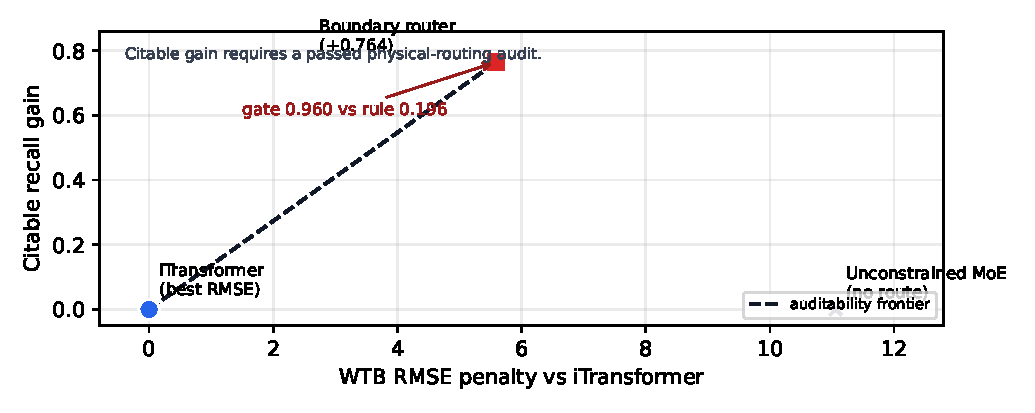
\includegraphics[width=0.9\linewidth,height=\textheight,keepaspectratio,alt={Accountability value versus forecasting RMSE price. Citable degraded-label gain is assigned only after the physical-routing audit passes. }]{artifacts/final_evidence_package/export/figures/accountability_tradeoff_curve.pdf}
\caption{Accountability value versus forecasting RMSE price. Citable
degraded-label gain is assigned only after the physical-routing audit
passes. \label{fig:accountability-tradeoff}}
\end{figure}

\begin{figure}
\centering
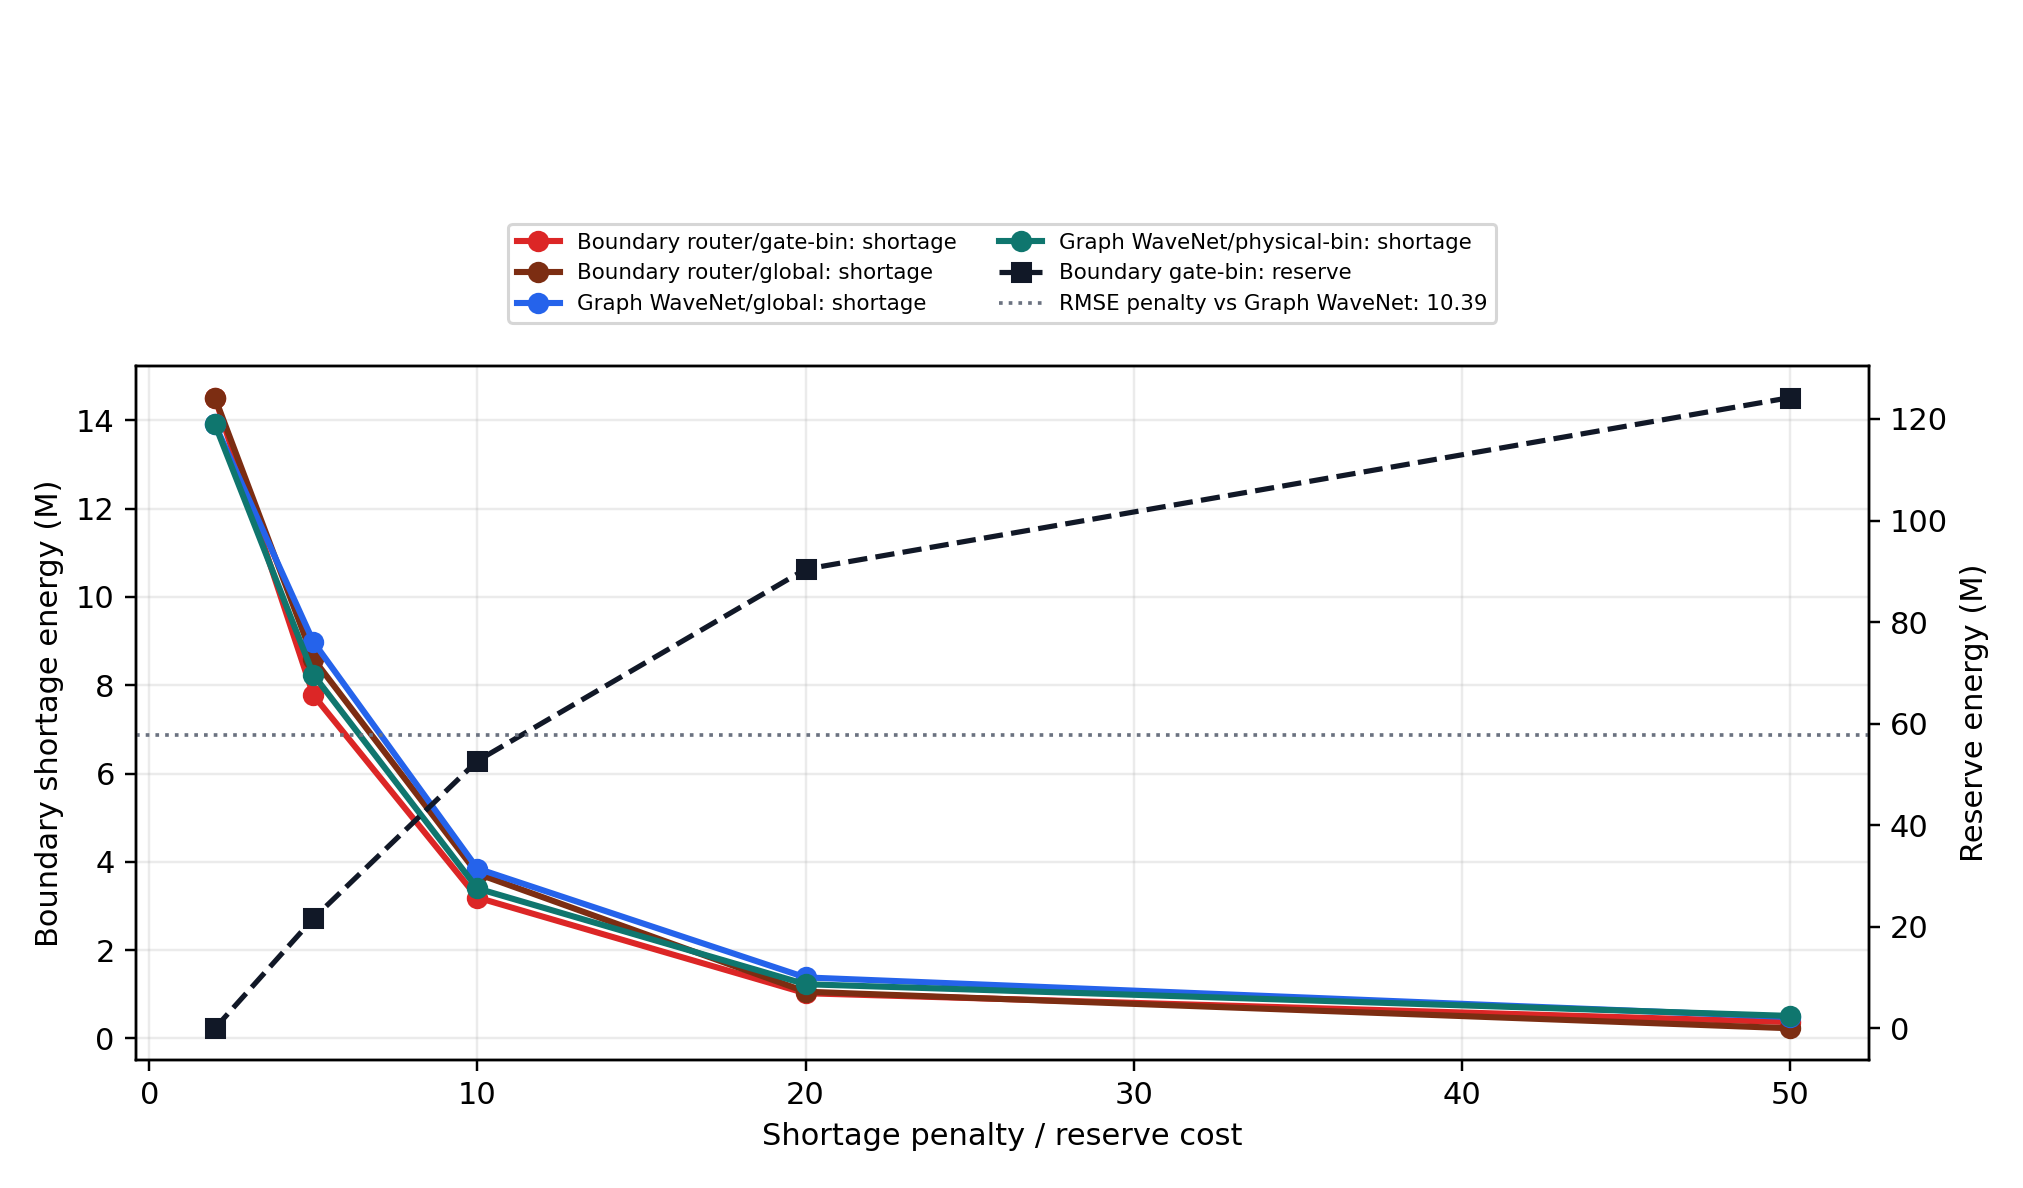
\includegraphics[width=0.92\linewidth,height=\textheight,keepaspectratio,alt={The decision curve places the reserve benefit beside the measured RMSE price. Gate-conditioned allocation is attractive only where the transition-window shortage reduction is worth the added reserve energy.}]{artifacts/final_evidence_package/export/figures/operational_decision_curve.png}
\caption{The decision curve places the reserve benefit beside the
measured RMSE price. Gate-conditioned allocation is attractive only
where the transition-window shortage reduction is worth the added
reserve energy.}
\end{figure}

\subsection{What Are the Costs and Deployment
Gates?}\label{what-are-the-costs-and-deployment-gates}

The accuracy cost is real and should be read as part of the design.
Graph WaveNet and lag-feature baselines remain better whole-sample
forecasters on WTB. The routed model is used when an operator or analyst
needs an accountable operating-state assignment that can feed a
boundary-specific decision, not when the sole target is minimum average
error. Time-forward testing gives the same message in another form:
late-period routing agreement remains high, but late-test RMSE rises
sharply, showing that stable semantics do not guarantee stable value
prediction under distribution shift.

The external wind-farm tests define the deployment gate.
Kelmarsh/Penmanshiel checks do not pass the held-out routing criterion,
identifying the conditions that must be verified before cross-farm use:
pitch or proxy observability, boundary-cell support, compatible turbine
geometry, local threshold estimation, and a held-out routing pass. The
method exports an evidence protocol, not a promise of automatic
transfer.

\begin{table}[H]
\centering
\footnotesize
\setlength{\tabcolsep}{4pt}
\renewcommand{\arraystretch}{1.08}
\caption{External-site deployment gates identified by Kelmarsh/Penmanshiel testing.}
\begin{tabularx}{0.98\linewidth}{>{\raggedright\arraybackslash}p{0.28\linewidth} >{\raggedright\arraybackslash}p{0.38\linewidth} >{\raggedright\arraybackslash}X}
\toprule
Gate & Observed evidence & Required decision before reserve use \\
\midrule
Held-out routing criterion & Default WTB boundary gives mean external NMI 0.4877, below the 0.50 criterion & Re-establish routing agreement locally \\
Local boundary recalibration & Average test NMI changes from 0.1324 to 0.1491 after validation-only recalibration & Treat threshold transfer as insufficient \\
Pitch/proxy observability & One transfer direction has no effective pitch-feature coverage or boundary cells & Require pitch channels or a validated proxy \\
Calibration-window adaptation & Small-window adaptation remains below the held-out balanced-accuracy threshold & Use calibration only after a held-out pass \\
Geometry and regime support & Farm scale, sensor fields, power curves, and regime shares differ across sites & Run a local evidence protocol before gate-bin reserve allocation \\
\bottomrule
\end{tabularx}
\end{table}

The WTB internal proxy drill shows the minimum evidence sequence: verify
sensor coverage, re-estimate local boundary and gate-to-regime map, pass
held-out routing, then run the reserve diagnostic. Stronger gate repair
is justified only when the reserve-window benefit exceeds the measured
RMSE and reserve-energy cost.

\begin{figure}
\centering
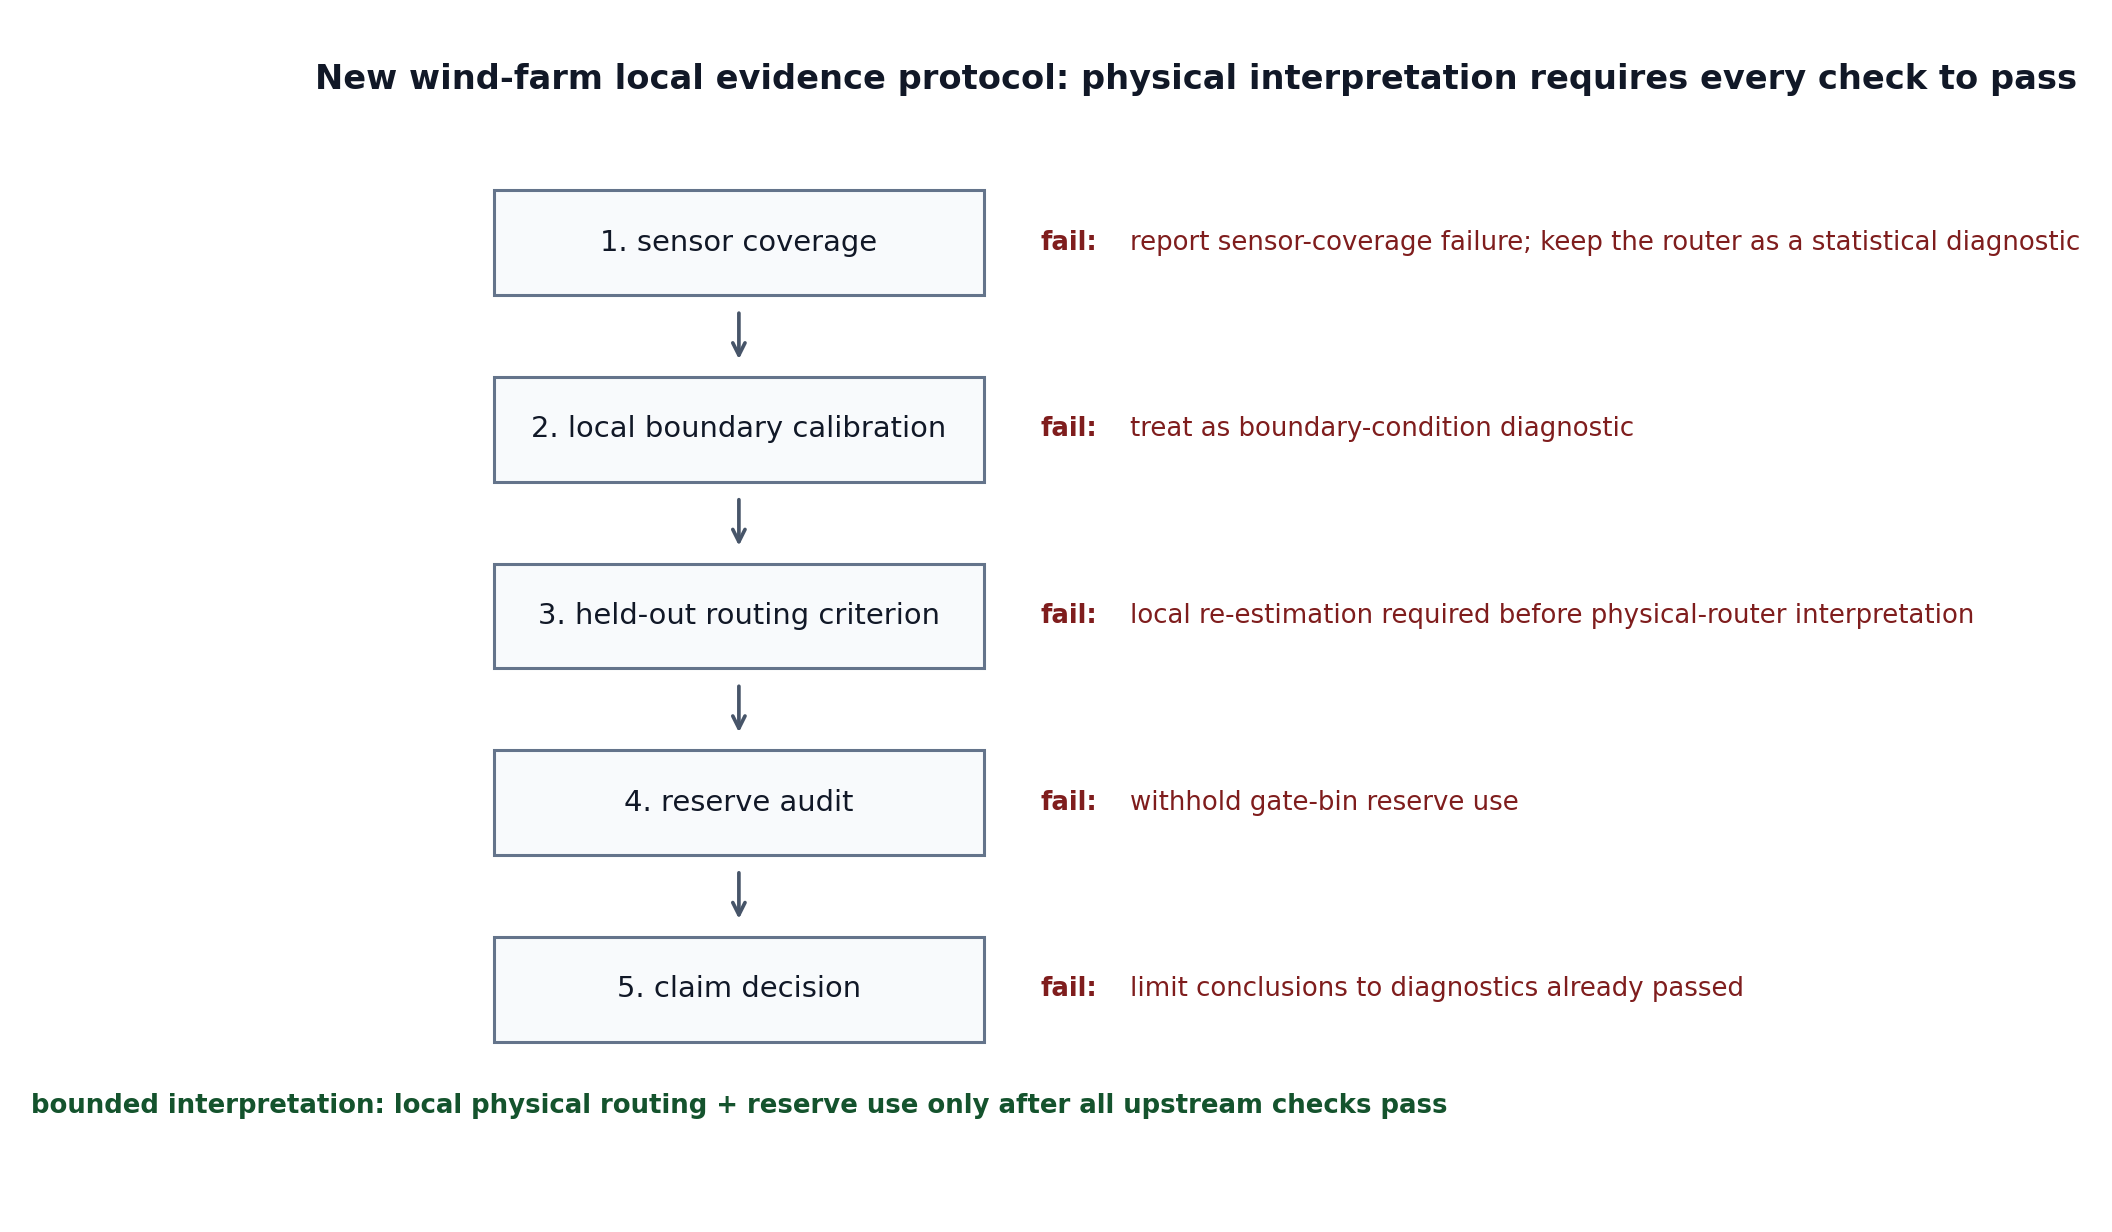
\includegraphics[width=0.94\linewidth,height=\textheight,keepaspectratio,alt={The new-site protocol turns external failure into a practical safety check: sensor coverage, local boundary calibration, held-out routing, and reserve audit must all pass before gate-conditioned reserve allocation is used.}]{artifacts/final_evidence_package/export/figures/new_wind_farm_deployment_checklist.png}
\caption{The new-site protocol turns external failure into a practical
safety check: sensor coverage, local boundary calibration, held-out
routing, and reserve audit must all pass before gate-conditioned reserve
allocation is used.}
\end{figure}

\section{Limitations}\label{limitations}

The WTB correction depends on threshold-based pseudo-labels derived from
wind speed and mean pitch angle. Those same channels also appear in the
gate anchor, so the method deliberately constrains the router to a
declared operating boundary. The label-degradation audit shows value
under delayed, missing, or noisy labels, but it should not be read as
anchor-free physical discovery or as a general future-label switch
predictor. The claim is boundary-aware regularized routing that remains
useful when the operational label stream degrades.

The active-power anchor has a strict timing requirement. \texttt{Patv}
is allowed only as the historical/anchor-time active-power measurement
available when the forecast is issued; future active power remains the
supervised target. This is a defensible SCADA forecasting convention,
but it is also a portability constraint. The five-seed anchor-stress
evidence (Table 7) shows that removing \texttt{Patv} or
\texttt{Pab\_mean} individually leaves the gate essentially intact,
while lagging both channels lowers the mean NMI but still crosses the
0.65 threshold. If a deployment environment delays active-power
telemetry or changes channel definitions, the Patv anchor must be
removed or lagged and the leakage, intervention, and reserve diagnostics
must be rerun.

The expert-regime language is tied to the implemented logit convention.
The first primary-regime logits are fixed to the operating labels during
supervised alignment, which prevents seed-wise permutation for those
anchored meanings. That makes cross-seed MPPT/pitch statements
interpretable, but only for the anchored logits and only under the
declared mapping. Unassigned experts and wake auxiliary logits should
not be overread as universal turbine states.

The comparison is bounded. WTB includes graph, transformer, lag-feature,
persistence, power-curve, DLinear-style references, and
validation-frozen empirical quantile reserve baselines, while ERA5
includes persistence and several learned baselines. Larger time-series
backbones, broader graph-transformer variants, trained
quantile-regression forecasters, scenario reserve, distributional
reserve, and security-constrained reserve methods are outside the
present benchmark.

The reserve audit is a normalized proxy: fixed empirical quantile bins
calibrated on validation shortfall and tested once on held-out
predictions. It ranks boundary-window tradeoffs under declared cost
ratios, but it is not a market-price or security-constrained dispatch
study. External diagnostics fail the held-out routing criterion;
Kelmarsh/Penmanshiel testing identifies the sensor coverage, pitch
observability, local boundary re-estimation, and held-out routing checks
that must pass before cross-farm use. The time-forward audit shows that
late-period distribution shift preserves routing agreement while
degrading value prediction: the method supports routing semantics, not
time-stable forecasting accuracy.

Statistical reliability is uneven (Supplementary Table A6). The
strongest claims are the five-seed WTB routing-recovery,
mechanism-intervention, and within-WTB spatial/temporal stress results;
gate-alignment deltas versus the full MoE and boundary-window
reserve-cost comparisons remain bounded diagnostics, not superiority
claims.

\section{Conclusion}\label{conclusion}

This paper introduces SCADA-anchored regime-aware routing as an
auditable control-boundary framework for wind-turbine forecasting. The
boundary-forced router recovers the declared WTB MPPT-to-pitch partition
(NMI about 0.87, ARI about 0.92), keeps 0.960 early pitch-window recall
under a six-step label delay while the delayed threshold rule falls to
0.196, and exposes transition-window reserve risk. This accountability
has a measured accuracy price: overall RMSE 236.13 versus 225.74 for
Graph WaveNet. Validation-frozen quantile baselines, Supplementary Table
A6, and Kelmarsh/Penmanshiel deployment gates keep the claim bounded.
The contribution is not forecasting SOTA or universal reserve-policy
optimality, but an auditable MPPT-to-pitch routing tool with
degraded-label value, RMSE price, and explicit transfer conditions.

\section{Declaration of generative AI and AI-assisted technologies in
the manuscript preparation
process}\label{declaration-of-generative-ai-and-ai-assisted-technologies-in-the-manuscript-preparation-process}

During the preparation of this work, the authors used OpenAI
ChatGPT/Codex to support language editing, consistency checking, and
submission-material drafting. The tools were not used to generate data,
run analyses, create references, or determine scientific conclusions.
After using these tools, the authors reviewed and edited the content as
needed and take full responsibility for the content of the published
article.

\section{Code and data availability}\label{code-and-data-availability}

The raw datasets are publicly available: KDD Cup 2022, Kelmarsh, and
Penmanshiel SCADA records. Raw third-party data are not redistributed.
Code, configuration files, releasable derived tables, figure data, and
model checkpoints will be made available with the article. The
reproduction package includes end-to-end scripts for the WTB routing
analysis, reserve audit, anchor-stress cache/train/guard protocol,
anchor-stress early-warning label-degradation audit, and external
boundary diagnostics. The provenance package lists the anchor-stress
cache/train/guard and early-warning protocols as mandatory. The analysis
involves no human subjects.

\clearpage

\section*{References}\label{references}
\addcontentsline{toc}{section}{References}

\protect\phantomsection\label{refs}
\begin{CSLReferences}{0}{0}
\bibitem[\citeproctext]{ref-wu2019graphwavenet}
\CSLLeftMargin{{[}1{]} }%
\CSLRightInline{Wu, Z., Pan, S., Long, G., Jiang, J., Zhang, C.,
\emph{Graph WaveNet for deep spatial-temporal graph modeling},
\emph{Proceedings of the 28th international joint conference on
artificial intelligence} 1907--1913;2019,
doi:\href{https://doi.org/10.24963/ijcai.2019/264}{10.24963/ijcai.2019/264}.}

\bibitem[\citeproctext]{ref-park2019physicsinduced}
\CSLLeftMargin{{[}2{]} }%
\CSLRightInline{Park, J., Park, J., Physics-induced graph neural
network: An application to wind-farm power estimation, \emph{Energy}
187, 115883;2019,
doi:\href{https://doi.org/10.1016/j.energy.2019.115883}{10.1016/j.energy.2019.115883}.}

\bibitem[\citeproctext]{ref-yu2020sgnn}
\CSLLeftMargin{{[}3{]} }%
\CSLRightInline{Yu, M., Zhang, Z., Li, X., Yu, J., Gao, J., Liu, Z.,
You, B., Zheng, X., Yu, R., Superposition graph neural network for
offshore wind power prediction, \emph{Future Generation Computer
Systems} 113, 145--157;2020,
doi:\href{https://doi.org/10.1016/j.future.2020.06.024}{10.1016/j.future.2020.06.024}.}

\bibitem[\citeproctext]{ref-kim2024lidarscada}
\CSLLeftMargin{{[}4{]} }%
\CSLRightInline{Kim, D., Ryu, G., Moon, C., Accuracy of a short-term
wind power forecasting model based on deep learning using {LiDAR-SCADA}
integration: A case study of the 400-{MW} {Anholt} offshore wind farm,
\emph{Applied Energy} 373, 123882;2024,
doi:\href{https://doi.org/10.1016/j.apenergy.2024.123882}{10.1016/j.apenergy.2024.123882}.}

\bibitem[\citeproctext]{ref-daenens2025offshore}
\CSLLeftMargin{{[}5{]} }%
\CSLRightInline{Daenens, S., Verstraeten, T., Daems, P.-J., Nowé, A.,
Helsen, J., Spatio-temporal graph neural networks for power prediction
in offshore wind farms using SCADA data, \emph{Wind Energy Science} 10,
1137--1152;2025,
doi:\href{https://doi.org/10.5194/wes-10-1137-2025}{10.5194/wes-10-1137-2025}.}

\bibitem[\citeproctext]{ref-jacobs1991adaptive}
\CSLLeftMargin{{[}6{]} }%
\CSLRightInline{Jacobs, R.A., Jordan, M.I., Nowlan, S.J., Hinton, G.E.,
Adaptive mixtures of local experts, \emph{Neural Computation} 3,
79--87;1991,
doi:\href{https://doi.org/10.1162/neco.1991.3.1.79}{10.1162/neco.1991.3.1.79}.}

\bibitem[\citeproctext]{ref-jordan1994hierarchical}
\CSLLeftMargin{{[}7{]} }%
\CSLRightInline{Jordan, M.I., Jacobs, R.A., Hierarchical mixtures of
experts and the {EM} algorithm, \emph{Neural Computation} 6,
181--214;1994,
doi:\href{https://doi.org/10.1162/neco.1994.6.2.181}{10.1162/neco.1994.6.2.181}.}

\bibitem[\citeproctext]{ref-shazeer2017outrageously}
\CSLLeftMargin{{[}8{]} }%
\CSLRightInline{Shazeer, N., Mirhoseini, A., Maziarz, K., Davis, A., Le,
Q., Hinton, G., Dean, J., \emph{Outrageously large neural networks: The
sparsely-gated mixture-of-experts layer}, \emph{International conference
on learning representations} 2017,
\url{https://openreview.net/forum?id=B1ckMDqlg}.}

\bibitem[\citeproctext]{ref-fedus2022switch}
\CSLLeftMargin{{[}9{]} }%
\CSLRightInline{Fedus, W., Zoph, B., Shazeer, N., Switch transformers:
Scaling to trillion parameter models with simple and efficient sparsity,
\emph{Journal of Machine Learning Research} 23, 1--39;2022,
\url{https://www.jmlr.org/papers/v23/21-0998.html}.}

\bibitem[\citeproctext]{ref-shi2025timemoe}
\CSLLeftMargin{{[}10{]} }%
\CSLRightInline{{Shi, S., Han, L., Liu, Y., others}, \emph{Time-MoE:
Billion-scale time series foundation models with mixture of experts},
\emph{International conference on learning representations} 2025,
\url{https://arxiv.org/abs/2409.16040}.}

\bibitem[\citeproctext]{ref-pinson2013forecasting}
\CSLLeftMargin{{[}11{]} }%
\CSLRightInline{Pinson, P., Wind energy: Forecasting challenges for its
operational management, \emph{Statistical Science} 28, 564--585;2013,
doi:\href{https://doi.org/10.1214/13-STS445}{10.1214/13-STS445}.}

\bibitem[\citeproctext]{ref-wang2025uncertaintyreview}
\CSLLeftMargin{{[}12{]} }%
\CSLRightInline{Wang, Y., Zhang, F., Kou, H., Zou, R., Hu, Q., Wang, J.,
A review of predictive uncertainty modeling techniques and evaluation
metrics in probabilistic wind speed and wind power forecasting,
\emph{Applied Energy} 396, 126234;2025,
doi:\href{https://doi.org/10.1016/j.apenergy.2025.126234}{10.1016/j.apenergy.2025.126234}.}

\bibitem[\citeproctext]{ref-guo2019astgcn}
\CSLLeftMargin{{[}13{]} }%
\CSLRightInline{Guo, S., Lin, Y., Feng, N., Song, C., Wan, H.,
\emph{Attention based spatial-temporal graph convolutional networks for
traffic flow forecasting}, \emph{Proceedings of the AAAI conference on
artificial intelligence} 33, 922--929;2019,
doi:\href{https://doi.org/10.1609/aaai.v33i01.3301922}{10.1609/aaai.v33i01.3301922}.}

\bibitem[\citeproctext]{ref-bai2020agcrn}
\CSLLeftMargin{{[}14{]} }%
\CSLRightInline{Bai, L., Yao, L., Li, C., Wang, X., Wang, C.,
\emph{Adaptive graph convolutional recurrent network for traffic
forecasting}, \emph{Advances in neural information processing systems}
33, 17804--17815;2020.}

\bibitem[\citeproctext]{ref-karpatne2017tgds}
\CSLLeftMargin{{[}15{]} }%
\CSLRightInline{Karpatne, A., Atluri, G., Faghmous, J.H., Steinbach, M.,
Banerjee, A., Ganguly, A., Shekhar, S., Samatova, N.F., Kumar, V.,
Theory-guided data science: A new paradigm for scientific discovery from
data, \emph{IEEE Transactions on Knowledge and Data Engineering} 29,
2318--2331;2017,
doi:\href{https://doi.org/10.1109/TKDE.2017.2720168}{10.1109/TKDE.2017.2720168}.}

\bibitem[\citeproctext]{ref-karniadakis2021piml}
\CSLLeftMargin{{[}16{]} }%
\CSLRightInline{Karniadakis, G.E., Kevrekidis, I.G., Lu, L., Perdikaris,
P., Wang, S., Yang, L., Physics-informed machine learning, \emph{Nature
Reviews Physics} 3, 422--440;2021,
doi:\href{https://doi.org/10.1038/s42254-021-00314-5}{10.1038/s42254-021-00314-5}.}

\bibitem[\citeproctext]{ref-parsa2025pimlreview}
\CSLLeftMargin{{[}17{]} }%
\CSLRightInline{Parsa, S.M., Physics-informed machine learning meets
renewable energy systems: A review of advances, challenges, guidelines,
and future outlooks, \emph{Applied Energy} 402, 126925;2025,
doi:\href{https://doi.org/10.1016/j.apenergy.2025.126925}{10.1016/j.apenergy.2025.126925}.}

\bibitem[\citeproctext]{ref-tautzweinert2017scada}
\CSLLeftMargin{{[}18{]} }%
\CSLRightInline{Tautz-Weinert, J., Watson, S.J., Using SCADA data for
wind turbine condition monitoring: A review, \emph{IET Renewable Power
Generation} 11, 382--394;2017,
doi:\href{https://doi.org/10.1049/iet-rpg.2016.0248}{10.1049/iet-rpg.2016.0248}.}

\bibitem[\citeproctext]{ref-zhou2024sdwpfdata}
\CSLLeftMargin{{[}19{]} }%
\CSLRightInline{Zhou, J., Lu, X., Xiao, Y., Tang, J., Su, J., Li, Y.,
Liu, J., Lyu, J., Ma, Y., Dou, D., SDWPF: A dataset for spatial dynamic
wind power forecasting over a large turbine array, \emph{Scientific
Data} 11, 649;2024,
doi:\href{https://doi.org/10.1038/s41597-024-03427-5}{10.1038/s41597-024-03427-5}.}

\bibitem[\citeproctext]{ref-doherty2005reserve}
\CSLLeftMargin{{[}20{]} }%
\CSLRightInline{Doherty, R., O'Malley, M., A new approach to quantify
reserve demand in systems with significant installed wind capacity,
\emph{IEEE Transactions on Power Systems} 20, 587--595;2005,
doi:\href{https://doi.org/10.1109/TPWRS.2005.846206}{10.1109/TPWRS.2005.846206}.}

\bibitem[\citeproctext]{ref-ela2011operatingreserves}
\CSLLeftMargin{{[}21{]} }%
\CSLRightInline{Ela, E., Milligan, M., Kirby, B., \emph{Operating
reserves and variable generation}, 2011,
doi:\href{https://doi.org/10.2172/1023095}{10.2172/1023095},
\url{https://www.osti.gov/biblio/1023095}.}

\bibitem[\citeproctext]{ref-bremnes2004quantile}
\CSLLeftMargin{{[}22{]} }%
\CSLRightInline{Bremnes, J.B., Probabilistic wind power forecasts using
local quantile regression, \emph{Wind Energy} 7, 47--54;2004,
doi:\href{https://doi.org/10.1002/we.107}{10.1002/we.107}.}

\bibitem[\citeproctext]{ref-zhang2014probabilisticreview}
\CSLLeftMargin{{[}23{]} }%
\CSLRightInline{Zhang, Y., Wang, J., Wang, X., Review on probabilistic
forecasting of wind power generation, \emph{Renewable and Sustainable
Energy Reviews} 32, 255--270;2014,
doi:\href{https://doi.org/10.1016/j.rser.2014.01.033}{10.1016/j.rser.2014.01.033}.}

\bibitem[\citeproctext]{ref-hersbach2020era5}
\CSLLeftMargin{{[}24{]} }%
\CSLRightInline{Hersbach, H., Bell, B., Berrisford, P., Hirahara, S.,
Horányi, A., Muñoz-Sabater, J., Nicolas, J., Peubey, C., Radu, R.,
Schepers, D., Simmons, A., Soci, C., Abdalla, S., Abellan, X., Balsamo,
G., Bechtold, P., Biavati, G., Bidlot, J.-R., Bonavita, M., De Chiara,
G., Dahlgren, P., Dee, D., Diamantakis, M., Dragani, R., Flemming, J.,
Forbes, R., Fuentes, M., Geer, A., Haimberger, L., Healy, S., Hogan, R.,
Hólm, E., Janisková, M., Keeley, S., Laloyaux, P., Lopez, P., Lupu, C.,
Radnoti, G., Rosnay, P. de, Rozum, I., Vamborg, F., Villaume, S.,
Thépaut, J.-N., The {ERA5} global reanalysis, \emph{Quarterly Journal of
the Royal Meteorological Society} 146, 1999--2049;2020,
doi:\href{https://doi.org/10.1002/qj.3803}{10.1002/qj.3803}.}

\end{CSLReferences}

\clearpage

\section*{Appendix A. Training and implementation
details}\label{appendix-a.-training-and-implementation-details}
\addcontentsline{toc}{section}{Appendix A. Training and implementation
details}

\subsection*{Training loop summary}\label{training-loop-summary}
\addcontentsline{toc}{subsection}{Training loop summary}

\begin{Shaded}
\begin{Highlighting}[]
\NormalTok{Algorithm A1  Physics{-}aligned MoE training}
\NormalTok{Input: history windows X, graph sequence A, targets Y, primary regime anchors R,}
\NormalTok{       auxiliary wake labels W (WTB only), model parameters theta}
\NormalTok{for each minibatch do}
\NormalTok{    Build node{-}level graph context from the precomputed graph tensors}
\NormalTok{    Encode X with the directed{-}diffusion GRU to obtain node context H}
\NormalTok{    Compute gate logits Z and soft routing probabilities G}
\NormalTok{    Compute expert forecasts and aggregate them with G}
\NormalTok{    Evaluate L\_pred}
\NormalTok{    If MoE mode is active:}
\NormalTok{        add L\_bal on top{-}K routing statistics}
\NormalTok{        add L\_align on valid primary regime anchors}
\NormalTok{        if WTB: add L\_force on MPPT/pitch samples}
\NormalTok{        if WTB: add L\_aux on wake labels}
\NormalTok{        add L\_smooth on the final graph snapshot}
\NormalTok{    Update theta with AdamW and mixed precision}
\NormalTok{end for}
\NormalTok{Select the checkpoint with the best validation RMSE}
\end{Highlighting}
\end{Shaded}

\subsection*{Model-family and supplementary evidence
index}\label{model-family-and-supplementary-evidence-index}
\addcontentsline{toc}{subsection}{Model-family and supplementary
evidence index}

\begin{table}[H]
\centering
\small
\setlength{\tabcolsep}{5pt}
\renewcommand{\arraystretch}{1.1}
\caption*{\textbf{Table A1.} In-family model comparison used for mechanism validation.}
\begin{tabularx}{0.98\textwidth}{>{\raggedright\arraybackslash}p{0.18\textwidth} >{\raggedright\arraybackslash}p{0.16\textwidth} >{\raggedright\arraybackslash}X >{\raggedright\arraybackslash}p{0.20\textwidth} >{\raggedright\arraybackslash}p{0.18\textwidth}}
\toprule
Model & Routing & Extra terms & Params & Role \\
\midrule
Dense (matched) & Single dense head & None & WTB 110,012 / ERA5 103,272 & Shared-mapping reference \\
Unconstrained MoE & Node-level soft gate & Prediction loss only & WTB 110,012 / ERA5 103,843 & Routed-capacity control \\
Corrected routing comparator & Node-level soft gate & WTB boundary-forced: $L_{bal}+L_{align}+L_{force}$; ERA5: full corrected stack & WTB 110,012 / ERA5 103,843 & Accountability comparator \\
\bottomrule
\end{tabularx}
\end{table}

\subsection*{Auxiliary losses}\label{auxiliary-losses}
\addcontentsline{toc}{subsection}{Auxiliary losses}

Let \(\mathcal{B}\) denote the routed samples after masks, with
\(B=|\mathcal{B}|\). The soft importance and normalized share of expert
\(e\) are \(I_e = \frac{1}{B}\sum_{n=1}^{B} g_n^{(e)}\) and
\(P_e = I_e / \sum_{r} I_r\). The top-\(K\) load is
\(f_e = \frac{1}{B}\sum_{n=1}^{B}\mathbf{1}[e \in \mathrm{TopK}(\mathbf{g}_n)]\),
giving \[\mathcal{L}_{\mathrm{bal}} = E\sum_{e=1}^{E} f_e P_e - 1.\] For
WTB wake supervision,
\[\mathcal{L}_{\mathrm{aux}} = \frac{1}{|\Omega_{\mathrm{wake}}|}\sum_{(i,t)\in\Omega_{\mathrm{wake}}}\mathrm{BCE}(z^{(\mathrm{wake})}_{i,t}, W_{i,t}),\]
where \(\Omega_{\mathrm{wake}}\) contains only MPPT and pitch-control
samples with defined wake flags. The graph-smoothness penalty is
\[\mathcal{L}_{\mathrm{smooth}} = \frac{\sum_{t\in\mathcal{T}_{\mathcal{B}}}\sum_{i,j}\mathcal{A}_t(i,j)\lVert\mathbf{g}_{i,t}-\mathbf{g}_{j,t}\rVert_2^2}{\sum_{t\in\mathcal{T}_{\mathcal{B}}}\sum_{i,j}\mathcal{A}_t(i,j)+\epsilon}.\]

\subsection*{Graph construction
details}\label{graph-construction-details}
\addcontentsline{toc}{subsection}{Graph construction details}

For WTB, the downstream unit vector is
\(\mathbf{u}_{i,t}=[\sin(\theta_{i,t}+\pi), \cos(\theta_{i,t}+\pi)]^{\top}\).
With \(\Delta\mathbf{p}_{ij}=\mathbf{p}_j-\mathbf{p}_i\), the streamwise
and cross-stream distances are
\(d^{\parallel}_{ij,t}=\Delta\mathbf{p}_{ij}^{\top}\mathbf{u}_{i,t}\)
and
\(d^{\perp}_{ij,t}=|\Delta p^x_{ij}u^y_{i,t}-\Delta p^y_{ij}u^x_{i,t}|\).
A candidate edge activates when
\[\mathbb{I}^{\mathrm{cone}}_{ij,t}=\mathbf{1}\!\left[d^{\parallel}_{ij,t}>0\;\land\;\arctan\!\left(\frac{d^{\perp}_{ij,t}}{\max(d^{\parallel}_{ij,t},10^{-6})}\right)\le\phi\right].\]
The wake weight is
\(\tilde{\mathcal{A}}_t(i,j)=\exp(-d^{\parallel}_{ij,t}/\alpha)\exp(-|d^{\perp}_{ij,t}|/\beta)\mathbb{I}^{\mathrm{cone}}_{ij,t}\).
If wind direction is missing, fall back to
\(\mathcal{A}^{\mathrm{static}}(i,j)=\exp(-\lVert\Delta\mathbf{p}_{ij}\rVert_2/d_{\max})\).
Only the strongest \(M\) inbound weights are retained. The wake score
and flag are \(s^{\mathrm{wake}}_{i,t}=\sum_{j}\mathcal{A}_t(i,j)\) and
\[W_{i,t}=\begin{cases}1,&s^{\mathrm{wake}}_{i,t}\ge q_{0.75}^{\mathrm{wake}}\land R^{\mathrm{wtb}}_{i,t}\in\{1,2\},\\0,&s^{\mathrm{wake}}_{i,t}<q_{0.75}^{\mathrm{wake}}\land R^{\mathrm{wtb}}_{i,t}\in\{1,2\},\\\varnothing,&\text{otherwise.}\end{cases}\]

For ERA5, the retained symmetric graph uses a Gaussian kernel on
great-circle distances:
\[\mathcal{A}(i,j)=\exp\!\left(-\frac{d_{ij}^2}{2\sigma^2}\right)\mathbf{1}[j\in\mathcal{N}_{k_{\mathrm{nn}}}(i)\;\text{or}\;i\in\mathcal{N}_{k_{\mathrm{nn}}}(j)],\]
where \(\sigma\) is the median retained neighbor distance on the
training graph.

\subsection*{Shared constants}\label{shared-constants}
\addcontentsline{toc}{subsection}{Shared constants}

\begin{table}[H]
\centering
\footnotesize
\setlength{\tabcolsep}{5pt}
\renewcommand{\arraystretch}{1.08}
\caption*{\textbf{Table A3.} Shared architecture, graph, and training constants used in the reported experiments.}
\begin{tabularx}{0.98\textwidth}{>{\raggedright\arraybackslash}p{0.30\textwidth} >{\raggedright\arraybackslash}p{0.18\textwidth} >{\raggedright\arraybackslash}p{0.18\textwidth} >{\raggedright\arraybackslash}X}
\toprule
Item & WTB & ERA5 & Role \\
\midrule
History / horizon $(H,P)$ & $(36,24)$ & $(36,24)$ & Input and forecast lengths \\
Gate softmax temperature $\tau$ & 0.7 & 0.7 & Soft routing sharpness \\
Top-$K$ in $L_{\mathrm{bal}}$ & 1 & 1 & Balancing statistic only \\
Hidden size $d$ & 64 & 64 & Shared encoder width \\
$k_{\mathrm{nn}}$ candidates & 8 & 8 & Initial neighborhood size \\
Maximum candidate radius $d_{\max}$ & 1500 m & not used & WTB proximity fallback / candidate filter \\
Wake-cone half-angle $\phi$ & $25^\circ$ & not used & WTB downstream activation \\
Streamwise decay $\alpha$ & 1200 m & not used & WTB wake attenuation \\
Cross-stream decay $\beta$ & 400 m & not used & WTB wake attenuation \\
Retained inbound edges $M$ & 5 & symmetric $k_{\mathrm{nn}}$ graph & Final graph sparsity \\
Optimizer & AdamW & AdamW & Shared optimizer \\
Learning rate & $2 \times 10^{-3}$ & $2 \times 10^{-3}$ & Shared schedule \\
Weight decay & $10^{-4}$ & $10^{-4}$ & Shared regularization \\
Batch size & 16 & 16 & Shared mini-batch size \\
Gradient clipping & 1.0 & 1.0 & Shared training stabilization \\
\bottomrule
\end{tabularx}
\end{table}

\subsection*{Dataset-specific thresholds and routing
weights}\label{dataset-specific-thresholds-and-routing-weights}
\addcontentsline{toc}{subsection}{Dataset-specific thresholds and
routing weights}

\begin{table}[H]
\centering
\footnotesize
\setlength{\tabcolsep}{5pt}
\renewcommand{\arraystretch}{1.08}
\caption*{\textbf{Table A4.} Dataset-specific regime thresholds used to construct routing anchors.}
\begin{tabularx}{0.98\textwidth}{>{\raggedright\arraybackslash}p{0.28\textwidth} >{\raggedright\arraybackslash}p{0.24\textwidth} >{\raggedright\arraybackslash}X}
\toprule
Dataset & Threshold & Value and meaning \\
\midrule
WTB & $u_{\mathrm{idle}}$ & 3.0 m s$^{-1}$, idle / active split \\
WTB & $u_{\mathrm{rated}}$ & 10.5 m s$^{-1}$, MPPT / pitch boundary \\
WTB & $p_{\mathrm{th}}$ & 2.0 deg, pitch-angle threshold \\
WTB & $q_{0.75}^{\mathrm{wake}}$ & 1.0690, upper-quartile wake-score threshold \\
ERA5 & $\varepsilon_{\mathrm{sshf}}$ & 169,116, 10th percentile of $|\texttt{sshf}|$ on the training split \\
ERA5 & $q_{0.95}^{\Delta}$ & 458,287.125, 95th percentile of $|\Delta\texttt{sshf}|$ on the training split \\
\bottomrule
\end{tabularx}
\end{table}

\begin{table}[H]
\centering
\footnotesize
\setlength{\tabcolsep}{6pt}
\renewcommand{\arraystretch}{1.08}
\caption*{\textbf{Table A5.} Active routing-loss weights in the reported corrected models.}
\begin{tabularx}{0.90\textwidth}{>{\raggedright\arraybackslash}p{0.18\textwidth} >{\centering\arraybackslash}p{0.18\textwidth} >{\centering\arraybackslash}p{0.18\textwidth} >{\raggedright\arraybackslash}X}
\toprule
Weight & WTB & ERA5 & Role \\
\midrule
$\lambda_{\mathrm{bal}}$ & 1000 & 0.01 & Expert-usage stabilization \\
$\lambda_{\mathrm{align}}$ & 5000 & 0.2 & Coarse regime alignment \\
$\lambda_{\mathrm{force}}$ & 10000 & 0 & Boundary-focused forcing \\
$\lambda_{\mathrm{aux}}$ & 250 & 0 & Wake-sensitive auxiliary routing \\
$\lambda_{\mathrm{smooth}}$ & 0.05 & 0.05 & Local routing coherence \\
\bottomrule
\end{tabularx}
\end{table}

\subsection*{Statistical claim
boundaries}\label{statistical-claim-boundaries}
\addcontentsline{toc}{subsection}{Statistical claim boundaries}

Table A6 records the reviewer-facing statistical boundary used for
wording. The RMSE price versus Graph WaveNet is FDR-significant,
gate-alignment deltas versus the full physics-aligned MoE are positive
but not FDR-significant, and boundary-window quantile reserve
comparisons have bootstrap intervals crossing zero. These tests are why
the main text uses price, diagnostic, and bounded-claim language rather
than forecast- or reserve-superiority wording.

\begin{table}[H]
\centering
\scriptsize
\setlength{\tabcolsep}{2.5pt}
\renewcommand{\arraystretch}{1.08}
\caption*{\textbf{Table A6.} Statistical claim boundaries used for reviewer-facing wording.}
\begin{tabularx}{\columnwidth}{>{\raggedright\arraybackslash}p{0.25\columnwidth} >{\centering\arraybackslash}p{0.13\columnwidth} >{\centering\arraybackslash}p{0.15\columnwidth} >{\centering\arraybackslash}p{0.11\columnwidth} >{\raggedright\arraybackslash}X}
\toprule
Claim & Estimate & 95\% CI & $p_{\mathrm{BH}}$ & Wording consequence \\
\midrule
Accuracy price vs Graph WaveNet & 9.029 & -- & <0.001 & Boundary router is significantly worse on headline RMSE \\
Boundary-band accuracy price & 17.758 & -- & 0.001 & The price also appears in the boundary window \\
Gate NMI vs full physics-aligned MoE & 0.040 & [0.008, 0.071] & 0.066 & Positive but not FDR-significant; cite as bounded mechanism contrast \\
Gate ARI vs full physics-aligned MoE & 0.035 & [-0.000, 0.078] & 0.126 & Positive but not FDR-significant; avoid superiority wording \\
Boundary quantile cost vs GWN physical bin & -0.263M & [-10.704M, 9.782M] & -- & CI crosses zero; reserve cost should remain a diagnostic claim \\
Boundary quantile violation vs GWN physical bin & 0.003 & [-0.011, 0.020] & -- & CI crosses zero; no universal reserve-policy optimality claim \\
\bottomrule
\end{tabularx}
\end{table}

\end{document}
